\documentclass[runningheads]{llncs}
\usepackage[english]{babel}
\usepackage[utf8]{inputenc}
% Carácteres especiales
\usepackage{fontenc}
% More advance packages

\usepackage{amssymb,amsbsy,mathrsfs,rotating,float,multirow,upgreek,amsmath,lineno,bm}

\usepackage{listings}
\usepackage{pgfplots}
\usepackage{tikz}
\usepgfplotslibrary{groupplots}
\usepackage{longtable}
\setlength{\LTcapwidth}{6in}
\usepackage[utf8]{inputenc}
\usepackage{epsfig,epic,eepic,threeparttable,amscd,here,lscape,tabularx,graphicx }
\usepackage{booktabs}
\usepackage{tabu,array}
\usepackage{overpic}
\usepackage{microtype}
%%%%%%%%%%%
%\usepackage{newtxtext,newtxmath}

%%%%%%%%%%%
\usepackage{caption}
\usepackage{subcaption}
% Permite ver y configurar los parámetros de la página
\usepackage{layout}
%Hyperref permite ver las secciones del texto
\usepackage[hidelinks]{hyperref}
\usepackage[noabbrev,capitalize]{cleveref}

\usepackage{nomencl}

\providecommand{\ppunto}[2]{\langle#1, #2 \rangle}% producto punto
\providecommand{\promed}[1]{{\mathbb{E}}\left\lbrace #1\right\rbrace}% operador de promedio
\providecommand{\promeddd}[2]{\mathbb{E}_{#1}\!\left\{#2\right\}}% op{\tiny }erador de promedio
\providecommand{\promedd}[2]{\mathds{E}_{#1}\left\{#2\right\}}% operador de promedio
\providecommand{\cov}[2]{{\fam=7 cov}\{#1, #2\}}% operador de covarianza
\providecommand{\gaus}[2]{{\fam=6 N}(#1 #2)} % FDP Gauss
% Kronecker delta function
\providecommand{\Kronecker}[2]{\delta_{K}( #1 , #2 )}
% cardinality
\providecommand{\Cardinality}[1]{| #1 |}



\providecommand{\est}[1]{{\widetilde {#1}}}
\providecommand{\s}[1]{\negthickspace#1\negthickspace}%
\newcolumntype{C}[1]{>{\centering}m{#1}}
\newcommand{\subconj}{\negthinspace\subset\negthinspace }
\newcommand{\en}{\negthinspace\in\negthinspace }
\newcommand{\igual}{\negthinspace=\negthinspace}
\newcommand{\dos}{\negthinspace:\negthinspace}

\newcommand{\Real}{\mathbb{R}}
\newcommand{\Natural}{\mathbb{N}}

\newcommand{\Tr}[1]{Tr \left( #1 \right)}
\newcommand{\diag}[1]{diag \left( #1 \right)}

\newcommand{\func}[1]{\mathcal {#1}}

\newcommand{\ve}[1]{\bm {#1}}
\newcommand{\mat}[1]{\bm {#1}}

\newenvironment{reviewer}{\setcounter{pointcounter}{1}}{}
\newcommand{\changes}[1]{\textcolor[rgb]{1.00,0.00,0.00}{#1}}
\newcommand{\point}[1]{\medskip \noindent
 \textsl{{\fontseries{b}\selectfont Point \thepointcounter}.
 \stepcounter{pointcounter} #1}}
\newcommand{\reply}{\medskip \noindent \textbf{Response}.\ }
\newcommand{\initresponses}{\newcounter{pointcounter}}
\newcommand*{\captionsource}[2]{%
  \caption[{#1}]{%
    #1%
    \\\hspace{\linewidth}%
    \textbf{Source:} #2%
  }%
}

\providecommand{\am}[1]{\textcolor{green}{#1}}
\providecommand{\dg}[1]{\textcolor{blue}{#1}}
%
\begin{document}
Dear PhD Austin J. Brockmeier

We truly appreciate all the valuable comments and recommendations provided. We thank you for the extensive revision of the manuscript. Your insights have been crucial in improving the quality and clarity of the work. Changes made on the document can be found in \changes{red color}. Our point-to-point responses to the reviewers' comments are given below:

\initresponses

\begin{reviewer}

\point{Overall the introduction and background is comprehensive and thorough with references. The proposed approach seems well founded and results are extensive.}

\reply{We appreciate your recognition and We are pleased to hear that you found the manuscript comprehensive and thorough with appropriate references.}


\point{here are some concerns with the baselines not being as competitive. Ablation study of spectral filtering is needed or allowing spectral filtering for other FC baselines would be useful.}

\reply{Thank you for your comment. We acknowledge that the document was not clear about both PLV and CCF being compared using the same frequency bands and time windows as specified in equation (5-6). To address this, we have revised the first two sentences of the experimental setup for clarity. The updated text is as follows:

\changes{
({i}) Preprocessing and trial-based extraction of \textit{s-t-f} representations. For extracting the subject EEG dynamics over time accurately, the sliding window length of feature extraction is fixed to the next values: $\tau=[0.5,1.0,1.5,2.0]$\,{s}, having an overlap of $75\%$. Additionally, similar to authors in \cite{ang2008filter} the frequency bands of interest are selected with the lower frequency limit set at 4 Hz, the upper limit set to 40 Hz, and an overlap of $50\%$. \cite{ang2008filter}
}
\changes{
({ii}) The estimation of the single-trial functional connectivity from the extracted \textit{s-t-f} features. For comparison, the proposed KCS-FC is contrasted with two commonly used single-trial FC measures. To facilitate this comparison, the KCS-FC in Equation~\eqref{eq:SRC} is interchanged with new single-trial FC measures. These measures can be estimated from a frequency $n$, a time window $w_t$, and a pair of channels ${cc'}$ (with $c \neq c'$, for all $cc'$ in $C$) as described in~\cite{rodrigue2019}.
\begin{equation}
			\rho(\ve{x}^{c}_{rnw_t},\ve{x}^{c'}_{rnw_t}) ={\left<\ve{x}^{c}_{rnw_t},\ve{x}^{c'}_{rnw_t}\right>}\label{Eq:Pearson}
\end{equation}
\begin{equation}		 
	{\Delta\phi(\ve{x}^{c}_{rnw_t},\ve{x}^{c}_{rnw_t})}  {= {|\exp(j(\ve{\phi}_{rnw_t}^{c}-\ve{\phi}_{rnw_t}^{c}))|}} \label{Eq:PLV} 
\end{equation}
} 
}

\point{One major concern is the validating of the hyper-parameter selection. Many times it is suggested that the 'best' is chosen. Is the 10-fold cross-validation split (mentioned on page 57) for trails or subjects? If the cross-validation is used how is the hyper-parameter search done? On the first split, or internally in each split, or only after all splits (test) are seen? If it is the latter than the hyper-parameter selection runs the risk of overfitting a dataset. and On page 68 it is clear that the split is done for trials of a subject.  However, it is not clear from the text whether the hyper-parameter, but "GridSearchCV" is mentioned. But this uses a gridsearch based on the CV performance meaning it gives the best hyper-parameters after all test splits are seen. Again, a more rigorous way is to do internal hyper-parameter selection. This may be a common issue with the other baselines too—I've reviewed papers at top tier venues where this is brought up and papers are rejected due to this invalid hyper-parameter selection approach.  In any case, the thesis should make this caveat clear.}

\reply{Thank you for your insight, we understand the concern about hyper-parameters overfitting. However, dDue to the low number of samples, we couldn't afford a nested cross-validation strategy. Instead, we used a 5-fold cross-validation at the subject level. While our approach doesn't completely eliminate overfitting risks, the small number of parameters in our model reduces this risk. Future work should focus on assessing model stability to overfitting with more robust validation techniques. EEG MI data has high intra-subject variability, significantly affecting training and testing sets. Our validation strategy follows the schema in \cite{schirrmeister2017deep}. Moreover, to check hyper-parameter sensitivity, we include the next two figure containing the CV mean test accuracy across all subjects for models KCS-FCnet and RKCS-FCnet.
\begin{figure}[h!]
  \centering
  \resizebox{\linewidth}{!}{% This file was created with tikzplotlib v0.10.1.
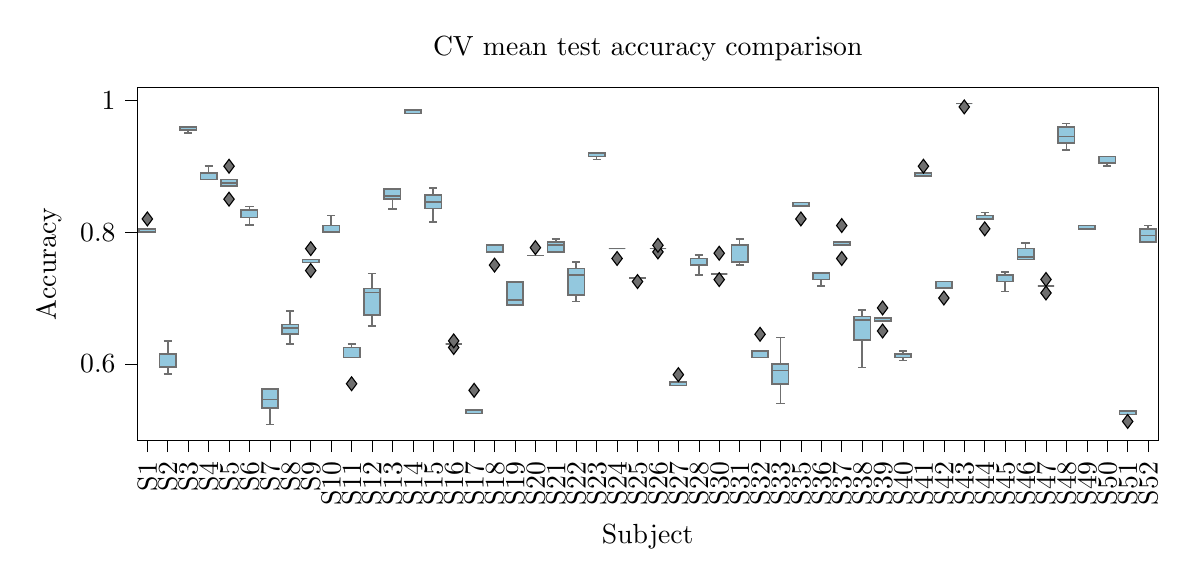
\begin{tikzpicture}

\definecolor{darkgray176}{RGB}{176,176,176}
\definecolor{dimgray111}{RGB}{111,111,111}
\definecolor{skyblue147200222}{RGB}{147,200,222}

\begin{axis}[
tick align=outside,
tick pos=left,
width=1.2\textwidth,
height=0.5\textwidth,
title={CV mean test accuracy comparison},
x grid style={darkgray176},
xlabel={Subject},
xmin=-0.5, xmax=49.5,
xtick style={color=black},
xtick={0,1,2,3,4,5,6,7,8,9,10,11,12,13,14,15,16,17,18,19,20,21,22,23,24,25,26,27,28,29,30,31,32,33,34,35,36,37,38,39,40,41,42,43,44,45,46,47,48,49},
xticklabel style={rotate=90.0,anchor=east},
xticklabels={
  S1,
  S2,
  S3,
  S4,
  S5,
  S6,
  S7,
  S8,
  S9,
  S10,
  S11,
  S12,
  S13,
  S14,
  S15,
  S16,
  S17,
  S18,
  S19,
  S20,
  S21,
  S22,
  S23,
  S24,
  S25,
  S26,
  S27,
  S28,
  S30,
  S31,
  S32,
  S33,
  S35,
  S36,
  S37,
  S38,
  S39,
  S40,
  S41,
  S42,
  S43,
  S44,
  S45,
  S46,
  S47,
  S48,
  S49,
  S50,
  S51,
  S52
},
y grid style={darkgray176},
ylabel={Accuracy},
ymin=0.484, ymax=1.01933333333333,
ytick style={color=black}
]
\path [draw=dimgray111, fill=skyblue147200222, semithick]
(axis cs:-0.4,0.8)
--(axis cs:0.4,0.8)
--(axis cs:0.4,0.805)
--(axis cs:-0.4,0.805)
--(axis cs:-0.4,0.8)
--cycle;
\path [draw=dimgray111, fill=skyblue147200222, semithick]
(axis cs:0.6,0.595)
--(axis cs:1.4,0.595)
--(axis cs:1.4,0.615)
--(axis cs:0.6,0.615)
--(axis cs:0.6,0.595)
--cycle;
\path [draw=dimgray111, fill=skyblue147200222, semithick]
(axis cs:1.6,0.955)
--(axis cs:2.4,0.955)
--(axis cs:2.4,0.96)
--(axis cs:1.6,0.96)
--(axis cs:1.6,0.955)
--cycle;
\path [draw=dimgray111, fill=skyblue147200222, semithick]
(axis cs:2.6,0.88)
--(axis cs:3.4,0.88)
--(axis cs:3.4,0.89)
--(axis cs:2.6,0.89)
--(axis cs:2.6,0.88)
--cycle;
\path [draw=dimgray111, fill=skyblue147200222, semithick]
(axis cs:3.6,0.87)
--(axis cs:4.4,0.87)
--(axis cs:4.4,0.88)
--(axis cs:3.6,0.88)
--(axis cs:3.6,0.87)
--cycle;
\path [draw=dimgray111, fill=skyblue147200222, semithick]
(axis cs:4.6,0.822222222222222)
--(axis cs:5.4,0.822222222222222)
--(axis cs:5.4,0.833333333333333)
--(axis cs:4.6,0.833333333333333)
--(axis cs:4.6,0.822222222222222)
--cycle;
\path [draw=dimgray111, fill=skyblue147200222, semithick]
(axis cs:5.6,0.533333333333333)
--(axis cs:6.4,0.533333333333333)
--(axis cs:6.4,0.5625)
--(axis cs:5.6,0.5625)
--(axis cs:5.6,0.533333333333333)
--cycle;
\path [draw=dimgray111, fill=skyblue147200222, semithick]
(axis cs:6.6,0.645)
--(axis cs:7.4,0.645)
--(axis cs:7.4,0.66)
--(axis cs:6.6,0.66)
--(axis cs:6.6,0.645)
--cycle;
\path [draw=dimgray111, fill=skyblue147200222, semithick]
(axis cs:7.6,0.754166666666667)
--(axis cs:8.4,0.754166666666667)
--(axis cs:8.4,0.758333333333333)
--(axis cs:7.6,0.758333333333333)
--(axis cs:7.6,0.754166666666667)
--cycle;
\path [draw=dimgray111, fill=skyblue147200222, semithick]
(axis cs:8.6,0.8)
--(axis cs:9.4,0.8)
--(axis cs:9.4,0.81)
--(axis cs:8.6,0.81)
--(axis cs:8.6,0.8)
--cycle;
\path [draw=dimgray111, fill=skyblue147200222, semithick]
(axis cs:9.6,0.61)
--(axis cs:10.4,0.61)
--(axis cs:10.4,0.625)
--(axis cs:9.6,0.625)
--(axis cs:9.6,0.61)
--cycle;
\path [draw=dimgray111, fill=skyblue147200222, semithick]
(axis cs:10.6,0.674285714285714)
--(axis cs:11.4,0.674285714285714)
--(axis cs:11.4,0.714285714285714)
--(axis cs:10.6,0.714285714285714)
--(axis cs:10.6,0.674285714285714)
--cycle;
\path [draw=dimgray111, fill=skyblue147200222, semithick]
(axis cs:11.6,0.85)
--(axis cs:12.4,0.85)
--(axis cs:12.4,0.865)
--(axis cs:11.6,0.865)
--(axis cs:11.6,0.85)
--cycle;
\path [draw=dimgray111, fill=skyblue147200222, semithick]
(axis cs:12.6,0.98)
--(axis cs:13.4,0.98)
--(axis cs:13.4,0.985)
--(axis cs:12.6,0.985)
--(axis cs:12.6,0.98)
--cycle;
\path [draw=dimgray111, fill=skyblue147200222, semithick]
(axis cs:13.6,0.835897435897436)
--(axis cs:14.4,0.835897435897436)
--(axis cs:14.4,0.856410256410256)
--(axis cs:13.6,0.856410256410256)
--(axis cs:13.6,0.835897435897436)
--cycle;
\path [draw=dimgray111, fill=skyblue147200222, semithick]
(axis cs:14.6,0.63)
--(axis cs:15.4,0.63)
--(axis cs:15.4,0.63)
--(axis cs:14.6,0.63)
--(axis cs:14.6,0.63)
--cycle;
\path [draw=dimgray111, fill=skyblue147200222, semithick]
(axis cs:15.6,0.525)
--(axis cs:16.4,0.525)
--(axis cs:16.4,0.53)
--(axis cs:15.6,0.53)
--(axis cs:15.6,0.525)
--cycle;
\path [draw=dimgray111, fill=skyblue147200222, semithick]
(axis cs:16.6,0.77)
--(axis cs:17.4,0.77)
--(axis cs:17.4,0.78)
--(axis cs:16.6,0.78)
--(axis cs:16.6,0.77)
--cycle;
\path [draw=dimgray111, fill=skyblue147200222, semithick]
(axis cs:17.6,0.689655172413793)
--(axis cs:18.4,0.689655172413793)
--(axis cs:18.4,0.724137931034483)
--(axis cs:17.6,0.724137931034483)
--(axis cs:17.6,0.689655172413793)
--cycle;
\path [draw=dimgray111, fill=skyblue147200222, semithick]
(axis cs:18.6,0.764705882352941)
--(axis cs:19.4,0.764705882352941)
--(axis cs:19.4,0.764705882352941)
--(axis cs:18.6,0.764705882352941)
--(axis cs:18.6,0.764705882352941)
--cycle;
\path [draw=dimgray111, fill=skyblue147200222, semithick]
(axis cs:19.6,0.77)
--(axis cs:20.4,0.77)
--(axis cs:20.4,0.785)
--(axis cs:19.6,0.785)
--(axis cs:19.6,0.77)
--cycle;
\path [draw=dimgray111, fill=skyblue147200222, semithick]
(axis cs:20.6,0.705)
--(axis cs:21.4,0.705)
--(axis cs:21.4,0.745)
--(axis cs:20.6,0.745)
--(axis cs:20.6,0.705)
--cycle;
\path [draw=dimgray111, fill=skyblue147200222, semithick]
(axis cs:21.6,0.915)
--(axis cs:22.4,0.915)
--(axis cs:22.4,0.92)
--(axis cs:21.6,0.92)
--(axis cs:21.6,0.915)
--cycle;
\path [draw=dimgray111, fill=skyblue147200222, semithick]
(axis cs:22.6,0.775)
--(axis cs:23.4,0.775)
--(axis cs:23.4,0.775)
--(axis cs:22.6,0.775)
--(axis cs:22.6,0.775)
--cycle;
\path [draw=dimgray111, fill=skyblue147200222, semithick]
(axis cs:23.6,0.73)
--(axis cs:24.4,0.73)
--(axis cs:24.4,0.73)
--(axis cs:23.6,0.73)
--(axis cs:23.6,0.73)
--cycle;
\path [draw=dimgray111, fill=skyblue147200222, semithick]
(axis cs:24.6,0.775)
--(axis cs:25.4,0.775)
--(axis cs:25.4,0.775)
--(axis cs:24.6,0.775)
--(axis cs:24.6,0.775)
--cycle;
\path [draw=dimgray111, fill=skyblue147200222, semithick]
(axis cs:25.6,0.567567567567568)
--(axis cs:26.4,0.567567567567568)
--(axis cs:26.4,0.572972972972973)
--(axis cs:25.6,0.572972972972973)
--(axis cs:25.6,0.567567567567568)
--cycle;
\path [draw=dimgray111, fill=skyblue147200222, semithick]
(axis cs:26.6,0.75)
--(axis cs:27.4,0.75)
--(axis cs:27.4,0.76)
--(axis cs:26.6,0.76)
--(axis cs:26.6,0.75)
--cycle;
\path [draw=dimgray111, fill=skyblue147200222, semithick]
(axis cs:27.6,0.736)
--(axis cs:28.4,0.736)
--(axis cs:28.4,0.736)
--(axis cs:27.6,0.736)
--(axis cs:27.6,0.736)
--cycle;
\path [draw=dimgray111, fill=skyblue147200222, semithick]
(axis cs:28.6,0.755)
--(axis cs:29.4,0.755)
--(axis cs:29.4,0.78)
--(axis cs:28.6,0.78)
--(axis cs:28.6,0.755)
--cycle;
\path [draw=dimgray111, fill=skyblue147200222, semithick]
(axis cs:29.6,0.61)
--(axis cs:30.4,0.61)
--(axis cs:30.4,0.62)
--(axis cs:29.6,0.62)
--(axis cs:29.6,0.61)
--cycle;
\path [draw=dimgray111, fill=skyblue147200222, semithick]
(axis cs:30.6,0.57)
--(axis cs:31.4,0.57)
--(axis cs:31.4,0.6)
--(axis cs:30.6,0.6)
--(axis cs:30.6,0.57)
--cycle;
\path [draw=dimgray111, fill=skyblue147200222, semithick]
(axis cs:31.6,0.84)
--(axis cs:32.4,0.84)
--(axis cs:32.4,0.845)
--(axis cs:31.6,0.845)
--(axis cs:31.6,0.84)
--cycle;
\path [draw=dimgray111, fill=skyblue147200222, semithick]
(axis cs:32.6,0.728205128205128)
--(axis cs:33.4,0.728205128205128)
--(axis cs:33.4,0.738461538461538)
--(axis cs:32.6,0.738461538461538)
--(axis cs:32.6,0.728205128205128)
--cycle;
\path [draw=dimgray111, fill=skyblue147200222, semithick]
(axis cs:33.6,0.78)
--(axis cs:34.4,0.78)
--(axis cs:34.4,0.785)
--(axis cs:33.6,0.785)
--(axis cs:33.6,0.78)
--cycle;
\path [draw=dimgray111, fill=skyblue147200222, semithick]
(axis cs:34.6,0.635897435897436)
--(axis cs:35.4,0.635897435897436)
--(axis cs:35.4,0.671794871794872)
--(axis cs:34.6,0.671794871794872)
--(axis cs:34.6,0.635897435897436)
--cycle;
\path [draw=dimgray111, fill=skyblue147200222, semithick]
(axis cs:35.6,0.665)
--(axis cs:36.4,0.665)
--(axis cs:36.4,0.67)
--(axis cs:35.6,0.67)
--(axis cs:35.6,0.665)
--cycle;
\path [draw=dimgray111, fill=skyblue147200222, semithick]
(axis cs:36.6,0.61)
--(axis cs:37.4,0.61)
--(axis cs:37.4,0.615)
--(axis cs:36.6,0.615)
--(axis cs:36.6,0.61)
--cycle;
\path [draw=dimgray111, fill=skyblue147200222, semithick]
(axis cs:37.6,0.885)
--(axis cs:38.4,0.885)
--(axis cs:38.4,0.89)
--(axis cs:37.6,0.89)
--(axis cs:37.6,0.885)
--cycle;
\path [draw=dimgray111, fill=skyblue147200222, semithick]
(axis cs:38.6,0.715)
--(axis cs:39.4,0.715)
--(axis cs:39.4,0.725)
--(axis cs:38.6,0.725)
--(axis cs:38.6,0.715)
--cycle;
\path [draw=dimgray111, fill=skyblue147200222, semithick]
(axis cs:39.6,0.995)
--(axis cs:40.4,0.995)
--(axis cs:40.4,0.995)
--(axis cs:39.6,0.995)
--(axis cs:39.6,0.995)
--cycle;
\path [draw=dimgray111, fill=skyblue147200222, semithick]
(axis cs:40.6,0.82)
--(axis cs:41.4,0.82)
--(axis cs:41.4,0.825)
--(axis cs:40.6,0.825)
--(axis cs:40.6,0.82)
--cycle;
\path [draw=dimgray111, fill=skyblue147200222, semithick]
(axis cs:41.6,0.725)
--(axis cs:42.4,0.725)
--(axis cs:42.4,0.735)
--(axis cs:41.6,0.735)
--(axis cs:41.6,0.725)
--cycle;
\path [draw=dimgray111, fill=skyblue147200222, semithick]
(axis cs:42.6,0.758333333333333)
--(axis cs:43.4,0.758333333333333)
--(axis cs:43.4,0.775)
--(axis cs:42.6,0.775)
--(axis cs:42.6,0.758333333333333)
--cycle;
\path [draw=dimgray111, fill=skyblue147200222, semithick]
(axis cs:43.6,0.717948717948718)
--(axis cs:44.4,0.717948717948718)
--(axis cs:44.4,0.717948717948718)
--(axis cs:43.6,0.717948717948718)
--(axis cs:43.6,0.717948717948718)
--cycle;
\path [draw=dimgray111, fill=skyblue147200222, semithick]
(axis cs:44.6,0.935)
--(axis cs:45.4,0.935)
--(axis cs:45.4,0.96)
--(axis cs:44.6,0.96)
--(axis cs:44.6,0.935)
--cycle;
\path [draw=dimgray111, fill=skyblue147200222, semithick]
(axis cs:45.6,0.805128205128205)
--(axis cs:46.4,0.805128205128205)
--(axis cs:46.4,0.81025641025641)
--(axis cs:45.6,0.81025641025641)
--(axis cs:45.6,0.805128205128205)
--cycle;
\path [draw=dimgray111, fill=skyblue147200222, semithick]
(axis cs:46.6,0.905)
--(axis cs:47.4,0.905)
--(axis cs:47.4,0.915)
--(axis cs:46.6,0.915)
--(axis cs:46.6,0.905)
--cycle;
\path [draw=dimgray111, fill=skyblue147200222, semithick]
(axis cs:47.6,0.523076923076923)
--(axis cs:48.4,0.523076923076923)
--(axis cs:48.4,0.528205128205128)
--(axis cs:47.6,0.528205128205128)
--(axis cs:47.6,0.523076923076923)
--cycle;
\path [draw=dimgray111, fill=skyblue147200222, semithick]
(axis cs:48.6,0.785)
--(axis cs:49.4,0.785)
--(axis cs:49.4,0.805)
--(axis cs:48.6,0.805)
--(axis cs:48.6,0.785)
--cycle;
\addplot [semithick, dimgray111]
table {%
0 0.8
0 0.8
};
\addplot [semithick, dimgray111]
table {%
0 0.805
0 0.805
};
\addplot [semithick, dimgray111]
table {%
-0.2 0.8
0.2 0.8
};
\addplot [semithick, dimgray111]
table {%
-0.2 0.805
0.2 0.805
};
\addplot [black, mark=diamond*, mark size=2.5, mark options={solid,fill=dimgray111}, only marks]
table {%
0 0.82
};
\addplot [semithick, dimgray111]
table {%
1 0.595
1 0.585
};
\addplot [semithick, dimgray111]
table {%
1 0.615
1 0.635
};
\addplot [semithick, dimgray111]
table {%
0.8 0.585
1.2 0.585
};
\addplot [semithick, dimgray111]
table {%
0.8 0.635
1.2 0.635
};
\addplot [semithick, dimgray111]
table {%
2 0.955
2 0.95
};
\addplot [semithick, dimgray111]
table {%
2 0.96
2 0.96
};
\addplot [semithick, dimgray111]
table {%
1.8 0.95
2.2 0.95
};
\addplot [semithick, dimgray111]
table {%
1.8 0.96
2.2 0.96
};
\addplot [semithick, dimgray111]
table {%
3 0.88
3 0.88
};
\addplot [semithick, dimgray111]
table {%
3 0.89
3 0.9
};
\addplot [semithick, dimgray111]
table {%
2.8 0.88
3.2 0.88
};
\addplot [semithick, dimgray111]
table {%
2.8 0.9
3.2 0.9
};
\addplot [semithick, dimgray111]
table {%
4 0.87
4 0.87
};
\addplot [semithick, dimgray111]
table {%
4 0.88
4 0.88
};
\addplot [semithick, dimgray111]
table {%
3.8 0.87
4.2 0.87
};
\addplot [semithick, dimgray111]
table {%
3.8 0.88
4.2 0.88
};
\addplot [black, mark=diamond*, mark size=2.5, mark options={solid,fill=dimgray111}, only marks]
table {%
4 0.85
4 0.9
};
\addplot [semithick, dimgray111]
table {%
5 0.822222222222222
5 0.811111111111111
};
\addplot [semithick, dimgray111]
table {%
5 0.833333333333333
5 0.838888888888889
};
\addplot [semithick, dimgray111]
table {%
4.8 0.811111111111111
5.2 0.811111111111111
};
\addplot [semithick, dimgray111]
table {%
4.8 0.838888888888889
5.2 0.838888888888889
};
\addplot [semithick, dimgray111]
table {%
6 0.533333333333333
6 0.508333333333333
};
\addplot [semithick, dimgray111]
table {%
6 0.5625
6 0.5625
};
\addplot [semithick, dimgray111]
table {%
5.8 0.508333333333333
6.2 0.508333333333333
};
\addplot [semithick, dimgray111]
table {%
5.8 0.5625
6.2 0.5625
};
\addplot [semithick, dimgray111]
table {%
7 0.645
7 0.63
};
\addplot [semithick, dimgray111]
table {%
7 0.66
7 0.68
};
\addplot [semithick, dimgray111]
table {%
6.8 0.63
7.2 0.63
};
\addplot [semithick, dimgray111]
table {%
6.8 0.68
7.2 0.68
};
\addplot [semithick, dimgray111]
table {%
8 0.754166666666667
8 0.754166666666667
};
\addplot [semithick, dimgray111]
table {%
8 0.758333333333333
8 0.758333333333333
};
\addplot [semithick, dimgray111]
table {%
7.8 0.754166666666667
8.2 0.754166666666667
};
\addplot [semithick, dimgray111]
table {%
7.8 0.758333333333333
8.2 0.758333333333333
};
\addplot [black, mark=diamond*, mark size=2.5, mark options={solid,fill=dimgray111}, only marks]
table {%
8 0.741666666666667
8 0.775
};
\addplot [semithick, dimgray111]
table {%
9 0.8
9 0.8
};
\addplot [semithick, dimgray111]
table {%
9 0.81
9 0.825
};
\addplot [semithick, dimgray111]
table {%
8.8 0.8
9.2 0.8
};
\addplot [semithick, dimgray111]
table {%
8.8 0.825
9.2 0.825
};
\addplot [semithick, dimgray111]
table {%
10 0.61
10 0.61
};
\addplot [semithick, dimgray111]
table {%
10 0.625
10 0.63
};
\addplot [semithick, dimgray111]
table {%
9.8 0.61
10.2 0.61
};
\addplot [semithick, dimgray111]
table {%
9.8 0.63
10.2 0.63
};
\addplot [black, mark=diamond*, mark size=2.5, mark options={solid,fill=dimgray111}, only marks]
table {%
10 0.57
};
\addplot [semithick, dimgray111]
table {%
11 0.674285714285714
11 0.657142857142857
};
\addplot [semithick, dimgray111]
table {%
11 0.714285714285714
11 0.737142857142857
};
\addplot [semithick, dimgray111]
table {%
10.8 0.657142857142857
11.2 0.657142857142857
};
\addplot [semithick, dimgray111]
table {%
10.8 0.737142857142857
11.2 0.737142857142857
};
\addplot [semithick, dimgray111]
table {%
12 0.85
12 0.835
};
\addplot [semithick, dimgray111]
table {%
12 0.865
12 0.865
};
\addplot [semithick, dimgray111]
table {%
11.8 0.835
12.2 0.835
};
\addplot [semithick, dimgray111]
table {%
11.8 0.865
12.2 0.865
};
\addplot [semithick, dimgray111]
table {%
13 0.98
13 0.98
};
\addplot [semithick, dimgray111]
table {%
13 0.985
13 0.985
};
\addplot [semithick, dimgray111]
table {%
12.8 0.98
13.2 0.98
};
\addplot [semithick, dimgray111]
table {%
12.8 0.985
13.2 0.985
};
\addplot [semithick, dimgray111]
table {%
14 0.835897435897436
14 0.815384615384615
};
\addplot [semithick, dimgray111]
table {%
14 0.856410256410256
14 0.866666666666667
};
\addplot [semithick, dimgray111]
table {%
13.8 0.815384615384615
14.2 0.815384615384615
};
\addplot [semithick, dimgray111]
table {%
13.8 0.866666666666667
14.2 0.866666666666667
};
\addplot [semithick, dimgray111]
table {%
15 0.63
15 0.63
};
\addplot [semithick, dimgray111]
table {%
15 0.63
15 0.63
};
\addplot [semithick, dimgray111]
table {%
14.8 0.63
15.2 0.63
};
\addplot [semithick, dimgray111]
table {%
14.8 0.63
15.2 0.63
};
\addplot [black, mark=diamond*, mark size=2.5, mark options={solid,fill=dimgray111}, only marks]
table {%
15 0.625
15 0.635
};
\addplot [semithick, dimgray111]
table {%
16 0.525
16 0.525
};
\addplot [semithick, dimgray111]
table {%
16 0.53
16 0.53
};
\addplot [semithick, dimgray111]
table {%
15.8 0.525
16.2 0.525
};
\addplot [semithick, dimgray111]
table {%
15.8 0.53
16.2 0.53
};
\addplot [black, mark=diamond*, mark size=2.5, mark options={solid,fill=dimgray111}, only marks]
table {%
16 0.56
};
\addplot [semithick, dimgray111]
table {%
17 0.77
17 0.77
};
\addplot [semithick, dimgray111]
table {%
17 0.78
17 0.78
};
\addplot [semithick, dimgray111]
table {%
16.8 0.77
17.2 0.77
};
\addplot [semithick, dimgray111]
table {%
16.8 0.78
17.2 0.78
};
\addplot [black, mark=diamond*, mark size=2.5, mark options={solid,fill=dimgray111}, only marks]
table {%
17 0.75
};
\addplot [semithick, dimgray111]
table {%
18 0.689655172413793
18 0.689655172413793
};
\addplot [semithick, dimgray111]
table {%
18 0.724137931034483
18 0.724137931034483
};
\addplot [semithick, dimgray111]
table {%
17.8 0.689655172413793
18.2 0.689655172413793
};
\addplot [semithick, dimgray111]
table {%
17.8 0.724137931034483
18.2 0.724137931034483
};
\addplot [semithick, dimgray111]
table {%
19 0.764705882352941
19 0.764705882352941
};
\addplot [semithick, dimgray111]
table {%
19 0.764705882352941
19 0.764705882352941
};
\addplot [semithick, dimgray111]
table {%
18.8 0.764705882352941
19.2 0.764705882352941
};
\addplot [semithick, dimgray111]
table {%
18.8 0.764705882352941
19.2 0.764705882352941
};
\addplot [black, mark=diamond*, mark size=2.5, mark options={solid,fill=dimgray111}, only marks]
table {%
19 0.776470588235294
};
\addplot [semithick, dimgray111]
table {%
20 0.77
20 0.77
};
\addplot [semithick, dimgray111]
table {%
20 0.785
20 0.79
};
\addplot [semithick, dimgray111]
table {%
19.8 0.77
20.2 0.77
};
\addplot [semithick, dimgray111]
table {%
19.8 0.79
20.2 0.79
};
\addplot [semithick, dimgray111]
table {%
21 0.705
21 0.695
};
\addplot [semithick, dimgray111]
table {%
21 0.745
21 0.755
};
\addplot [semithick, dimgray111]
table {%
20.8 0.695
21.2 0.695
};
\addplot [semithick, dimgray111]
table {%
20.8 0.755
21.2 0.755
};
\addplot [semithick, dimgray111]
table {%
22 0.915
22 0.91
};
\addplot [semithick, dimgray111]
table {%
22 0.92
22 0.92
};
\addplot [semithick, dimgray111]
table {%
21.8 0.91
22.2 0.91
};
\addplot [semithick, dimgray111]
table {%
21.8 0.92
22.2 0.92
};
\addplot [semithick, dimgray111]
table {%
23 0.775
23 0.775
};
\addplot [semithick, dimgray111]
table {%
23 0.775
23 0.775
};
\addplot [semithick, dimgray111]
table {%
22.8 0.775
23.2 0.775
};
\addplot [semithick, dimgray111]
table {%
22.8 0.775
23.2 0.775
};
\addplot [black, mark=diamond*, mark size=2.5, mark options={solid,fill=dimgray111}, only marks]
table {%
23 0.76
};
\addplot [semithick, dimgray111]
table {%
24 0.73
24 0.73
};
\addplot [semithick, dimgray111]
table {%
24 0.73
24 0.73
};
\addplot [semithick, dimgray111]
table {%
23.8 0.73
24.2 0.73
};
\addplot [semithick, dimgray111]
table {%
23.8 0.73
24.2 0.73
};
\addplot [black, mark=diamond*, mark size=2.5, mark options={solid,fill=dimgray111}, only marks]
table {%
24 0.725
};
\addplot [semithick, dimgray111]
table {%
25 0.775
25 0.775
};
\addplot [semithick, dimgray111]
table {%
25 0.775
25 0.775
};
\addplot [semithick, dimgray111]
table {%
24.8 0.775
25.2 0.775
};
\addplot [semithick, dimgray111]
table {%
24.8 0.775
25.2 0.775
};
\addplot [black, mark=diamond*, mark size=2.5, mark options={solid,fill=dimgray111}, only marks]
table {%
25 0.77
25 0.78
};
\addplot [semithick, dimgray111]
table {%
26 0.567567567567568
26 0.567567567567568
};
\addplot [semithick, dimgray111]
table {%
26 0.572972972972973
26 0.572972972972973
};
\addplot [semithick, dimgray111]
table {%
25.8 0.567567567567568
26.2 0.567567567567568
};
\addplot [semithick, dimgray111]
table {%
25.8 0.572972972972973
26.2 0.572972972972973
};
\addplot [black, mark=diamond*, mark size=2.5, mark options={solid,fill=dimgray111}, only marks]
table {%
26 0.583783783783784
};
\addplot [semithick, dimgray111]
table {%
27 0.75
27 0.735
};
\addplot [semithick, dimgray111]
table {%
27 0.76
27 0.765
};
\addplot [semithick, dimgray111]
table {%
26.8 0.735
27.2 0.735
};
\addplot [semithick, dimgray111]
table {%
26.8 0.765
27.2 0.765
};
\addplot [semithick, dimgray111]
table {%
28 0.736
28 0.736
};
\addplot [semithick, dimgray111]
table {%
28 0.736
28 0.736
};
\addplot [semithick, dimgray111]
table {%
27.8 0.736
28.2 0.736
};
\addplot [semithick, dimgray111]
table {%
27.8 0.736
28.2 0.736
};
\addplot [black, mark=diamond*, mark size=2.5, mark options={solid,fill=dimgray111}, only marks]
table {%
28 0.728
28 0.768
};
\addplot [semithick, dimgray111]
table {%
29 0.755
29 0.75
};
\addplot [semithick, dimgray111]
table {%
29 0.78
29 0.79
};
\addplot [semithick, dimgray111]
table {%
28.8 0.75
29.2 0.75
};
\addplot [semithick, dimgray111]
table {%
28.8 0.79
29.2 0.79
};
\addplot [semithick, dimgray111]
table {%
30 0.61
30 0.61
};
\addplot [semithick, dimgray111]
table {%
30 0.62
30 0.62
};
\addplot [semithick, dimgray111]
table {%
29.8 0.61
30.2 0.61
};
\addplot [semithick, dimgray111]
table {%
29.8 0.62
30.2 0.62
};
\addplot [black, mark=diamond*, mark size=2.5, mark options={solid,fill=dimgray111}, only marks]
table {%
30 0.645
};
\addplot [semithick, dimgray111]
table {%
31 0.57
31 0.54
};
\addplot [semithick, dimgray111]
table {%
31 0.6
31 0.64
};
\addplot [semithick, dimgray111]
table {%
30.8 0.54
31.2 0.54
};
\addplot [semithick, dimgray111]
table {%
30.8 0.64
31.2 0.64
};
\addplot [semithick, dimgray111]
table {%
32 0.84
32 0.84
};
\addplot [semithick, dimgray111]
table {%
32 0.845
32 0.845
};
\addplot [semithick, dimgray111]
table {%
31.8 0.84
32.2 0.84
};
\addplot [semithick, dimgray111]
table {%
31.8 0.845
32.2 0.845
};
\addplot [black, mark=diamond*, mark size=2.5, mark options={solid,fill=dimgray111}, only marks]
table {%
32 0.82
};
\addplot [semithick, dimgray111]
table {%
33 0.728205128205128
33 0.717948717948718
};
\addplot [semithick, dimgray111]
table {%
33 0.738461538461538
33 0.738461538461539
};
\addplot [semithick, dimgray111]
table {%
32.8 0.717948717948718
33.2 0.717948717948718
};
\addplot [semithick, dimgray111]
table {%
32.8 0.738461538461539
33.2 0.738461538461539
};
\addplot [semithick, dimgray111]
table {%
34 0.78
34 0.78
};
\addplot [semithick, dimgray111]
table {%
34 0.785
34 0.785
};
\addplot [semithick, dimgray111]
table {%
33.8 0.78
34.2 0.78
};
\addplot [semithick, dimgray111]
table {%
33.8 0.785
34.2 0.785
};
\addplot [black, mark=diamond*, mark size=2.5, mark options={solid,fill=dimgray111}, only marks]
table {%
34 0.76
34 0.81
};
\addplot [semithick, dimgray111]
table {%
35 0.635897435897436
35 0.594871794871795
};
\addplot [semithick, dimgray111]
table {%
35 0.671794871794872
35 0.682051282051282
};
\addplot [semithick, dimgray111]
table {%
34.8 0.594871794871795
35.2 0.594871794871795
};
\addplot [semithick, dimgray111]
table {%
34.8 0.682051282051282
35.2 0.682051282051282
};
\addplot [semithick, dimgray111]
table {%
36 0.665
36 0.665
};
\addplot [semithick, dimgray111]
table {%
36 0.67
36 0.67
};
\addplot [semithick, dimgray111]
table {%
35.8 0.665
36.2 0.665
};
\addplot [semithick, dimgray111]
table {%
35.8 0.67
36.2 0.67
};
\addplot [black, mark=diamond*, mark size=2.5, mark options={solid,fill=dimgray111}, only marks]
table {%
36 0.65
36 0.685
};
\addplot [semithick, dimgray111]
table {%
37 0.61
37 0.605
};
\addplot [semithick, dimgray111]
table {%
37 0.615
37 0.62
};
\addplot [semithick, dimgray111]
table {%
36.8 0.605
37.2 0.605
};
\addplot [semithick, dimgray111]
table {%
36.8 0.62
37.2 0.62
};
\addplot [semithick, dimgray111]
table {%
38 0.885
38 0.885
};
\addplot [semithick, dimgray111]
table {%
38 0.89
38 0.89
};
\addplot [semithick, dimgray111]
table {%
37.8 0.885
38.2 0.885
};
\addplot [semithick, dimgray111]
table {%
37.8 0.89
38.2 0.89
};
\addplot [black, mark=diamond*, mark size=2.5, mark options={solid,fill=dimgray111}, only marks]
table {%
38 0.9
};
\addplot [semithick, dimgray111]
table {%
39 0.715
39 0.715
};
\addplot [semithick, dimgray111]
table {%
39 0.725
39 0.725
};
\addplot [semithick, dimgray111]
table {%
38.8 0.715
39.2 0.715
};
\addplot [semithick, dimgray111]
table {%
38.8 0.725
39.2 0.725
};
\addplot [black, mark=diamond*, mark size=2.5, mark options={solid,fill=dimgray111}, only marks]
table {%
39 0.7
};
\addplot [semithick, dimgray111]
table {%
40 0.995
40 0.995
};
\addplot [semithick, dimgray111]
table {%
40 0.995
40 0.995
};
\addplot [semithick, dimgray111]
table {%
39.8 0.995
40.2 0.995
};
\addplot [semithick, dimgray111]
table {%
39.8 0.995
40.2 0.995
};
\addplot [black, mark=diamond*, mark size=2.5, mark options={solid,fill=dimgray111}, only marks]
table {%
40 0.99
};
\addplot [semithick, dimgray111]
table {%
41 0.82
41 0.82
};
\addplot [semithick, dimgray111]
table {%
41 0.825
41 0.83
};
\addplot [semithick, dimgray111]
table {%
40.8 0.82
41.2 0.82
};
\addplot [semithick, dimgray111]
table {%
40.8 0.83
41.2 0.83
};
\addplot [black, mark=diamond*, mark size=2.5, mark options={solid,fill=dimgray111}, only marks]
table {%
41 0.805
};
\addplot [semithick, dimgray111]
table {%
42 0.725
42 0.71
};
\addplot [semithick, dimgray111]
table {%
42 0.735
42 0.74
};
\addplot [semithick, dimgray111]
table {%
41.8 0.71
42.2 0.71
};
\addplot [semithick, dimgray111]
table {%
41.8 0.74
42.2 0.74
};
\addplot [semithick, dimgray111]
table {%
43 0.758333333333333
43 0.758333333333333
};
\addplot [semithick, dimgray111]
table {%
43 0.775
43 0.783333333333333
};
\addplot [semithick, dimgray111]
table {%
42.8 0.758333333333333
43.2 0.758333333333333
};
\addplot [semithick, dimgray111]
table {%
42.8 0.783333333333333
43.2 0.783333333333333
};
\addplot [semithick, dimgray111]
table {%
44 0.717948717948718
44 0.717948717948718
};
\addplot [semithick, dimgray111]
table {%
44 0.717948717948718
44 0.717948717948718
};
\addplot [semithick, dimgray111]
table {%
43.8 0.717948717948718
44.2 0.717948717948718
};
\addplot [semithick, dimgray111]
table {%
43.8 0.717948717948718
44.2 0.717948717948718
};
\addplot [black, mark=diamond*, mark size=2.5, mark options={solid,fill=dimgray111}, only marks]
table {%
44 0.707692307692308
44 0.728205128205128
};
\addplot [semithick, dimgray111]
table {%
45 0.935
45 0.925
};
\addplot [semithick, dimgray111]
table {%
45 0.96
45 0.965
};
\addplot [semithick, dimgray111]
table {%
44.8 0.925
45.2 0.925
};
\addplot [semithick, dimgray111]
table {%
44.8 0.965
45.2 0.965
};
\addplot [semithick, dimgray111]
table {%
46 0.805128205128205
46 0.805128205128205
};
\addplot [semithick, dimgray111]
table {%
46 0.81025641025641
46 0.81025641025641
};
\addplot [semithick, dimgray111]
table {%
45.8 0.805128205128205
46.2 0.805128205128205
};
\addplot [semithick, dimgray111]
table {%
45.8 0.81025641025641
46.2 0.81025641025641
};
\addplot [semithick, dimgray111]
table {%
47 0.905
47 0.9
};
\addplot [semithick, dimgray111]
table {%
47 0.915
47 0.915
};
\addplot [semithick, dimgray111]
table {%
46.8 0.9
47.2 0.9
};
\addplot [semithick, dimgray111]
table {%
46.8 0.915
47.2 0.915
};
\addplot [semithick, dimgray111]
table {%
48 0.523076923076923
48 0.523076923076923
};
\addplot [semithick, dimgray111]
table {%
48 0.528205128205128
48 0.528205128205128
};
\addplot [semithick, dimgray111]
table {%
47.8 0.523076923076923
48.2 0.523076923076923
};
\addplot [semithick, dimgray111]
table {%
47.8 0.528205128205128
48.2 0.528205128205128
};
\addplot [black, mark=diamond*, mark size=2.5, mark options={solid,fill=dimgray111}, only marks]
table {%
48 0.512820512820513
};
\addplot [semithick, dimgray111]
table {%
49 0.785
49 0.785
};
\addplot [semithick, dimgray111]
table {%
49 0.805
49 0.81
};
\addplot [semithick, dimgray111]
table {%
48.8 0.785
49.2 0.785
};
\addplot [semithick, dimgray111]
table {%
48.8 0.81
49.2 0.81
};
\addplot [semithick, dimgray111]
table {%
-0.4 0.805
0.4 0.805
};
\addplot [semithick, dimgray111]
table {%
0.6 0.595
1.4 0.595
};
\addplot [semithick, dimgray111]
table {%
1.6 0.955
2.4 0.955
};
\addplot [semithick, dimgray111]
table {%
2.6 0.89
3.4 0.89
};
\addplot [semithick, dimgray111]
table {%
3.6 0.875
4.4 0.875
};
\addplot [semithick, dimgray111]
table {%
4.6 0.822222222222222
5.4 0.822222222222222
};
\addplot [semithick, dimgray111]
table {%
5.6 0.545833333333333
6.4 0.545833333333333
};
\addplot [semithick, dimgray111]
table {%
6.6 0.655
7.4 0.655
};
\addplot [semithick, dimgray111]
table {%
7.6 0.758333333333333
8.4 0.758333333333333
};
\addplot [semithick, dimgray111]
table {%
8.6 0.81
9.4 0.81
};
\addplot [semithick, dimgray111]
table {%
9.6 0.61
10.4 0.61
};
\addplot [semithick, dimgray111]
table {%
10.6 0.708571428571429
11.4 0.708571428571429
};
\addplot [semithick, dimgray111]
table {%
11.6 0.855
12.4 0.855
};
\addplot [semithick, dimgray111]
table {%
12.6 0.985
13.4 0.985
};
\addplot [semithick, dimgray111]
table {%
13.6 0.846153846153846
14.4 0.846153846153846
};
\addplot [semithick, dimgray111]
table {%
14.6 0.63
15.4 0.63
};
\addplot [semithick, dimgray111]
table {%
15.6 0.525
16.4 0.525
};
\addplot [semithick, dimgray111]
table {%
16.6 0.77
17.4 0.77
};
\addplot [semithick, dimgray111]
table {%
17.6 0.696551724137931
18.4 0.696551724137931
};
\addplot [semithick, dimgray111]
table {%
18.6 0.764705882352941
19.4 0.764705882352941
};
\addplot [semithick, dimgray111]
table {%
19.6 0.78
20.4 0.78
};
\addplot [semithick, dimgray111]
table {%
20.6 0.735
21.4 0.735
};
\addplot [semithick, dimgray111]
table {%
21.6 0.92
22.4 0.92
};
\addplot [semithick, dimgray111]
table {%
22.6 0.775
23.4 0.775
};
\addplot [semithick, dimgray111]
table {%
23.6 0.73
24.4 0.73
};
\addplot [semithick, dimgray111]
table {%
24.6 0.775
25.4 0.775
};
\addplot [semithick, dimgray111]
table {%
25.6 0.567567567567568
26.4 0.567567567567568
};
\addplot [semithick, dimgray111]
table {%
26.6 0.75
27.4 0.75
};
\addplot [semithick, dimgray111]
table {%
27.6 0.736
28.4 0.736
};
\addplot [semithick, dimgray111]
table {%
28.6 0.755
29.4 0.755
};
\addplot [semithick, dimgray111]
table {%
29.6 0.61
30.4 0.61
};
\addplot [semithick, dimgray111]
table {%
30.6 0.59
31.4 0.59
};
\addplot [semithick, dimgray111]
table {%
31.6 0.845
32.4 0.845
};
\addplot [semithick, dimgray111]
table {%
32.6 0.728205128205128
33.4 0.728205128205128
};
\addplot [semithick, dimgray111]
table {%
33.6 0.785
34.4 0.785
};
\addplot [semithick, dimgray111]
table {%
34.6 0.666666666666667
35.4 0.666666666666667
};
\addplot [semithick, dimgray111]
table {%
35.6 0.67
36.4 0.67
};
\addplot [semithick, dimgray111]
table {%
36.6 0.61
37.4 0.61
};
\addplot [semithick, dimgray111]
table {%
37.6 0.89
38.4 0.89
};
\addplot [semithick, dimgray111]
table {%
38.6 0.715
39.4 0.715
};
\addplot [semithick, dimgray111]
table {%
39.6 0.995
40.4 0.995
};
\addplot [semithick, dimgray111]
table {%
40.6 0.82
41.4 0.82
};
\addplot [semithick, dimgray111]
table {%
41.6 0.725
42.4 0.725
};
\addplot [semithick, dimgray111]
table {%
42.6 0.7625
43.4 0.7625
};
\addplot [semithick, dimgray111]
table {%
43.6 0.717948717948718
44.4 0.717948717948718
};
\addplot [semithick, dimgray111]
table {%
44.6 0.945
45.4 0.945
};
\addplot [semithick, dimgray111]
table {%
45.6 0.805128205128205
46.4 0.805128205128205
};
\addplot [semithick, dimgray111]
table {%
46.6 0.915
47.4 0.915
};
\addplot [semithick, dimgray111]
table {%
47.6 0.528205128205128
48.4 0.528205128205128
};
\addplot [semithick, dimgray111]
table {%
48.6 0.795
49.4 0.795
};
\end{axis}

\end{tikzpicture}
}
  \caption{Cross validation mean test accuracy comparison for KCS-FCnet model}
\end{figure}
The figure above shows the cross-validation mean test accuracy for different subjects using the KCS-FCnet model. It indicates that the mean test validation accuracy remains relatively consistent regardless of the hyper-parameters used, suggesting robustness to hyper-parameter variations.

\begin{figure}[h!]
  \centering
  \resizebox{\linewidth}{!}{\input{../Tesis_document/Figures/extras/test_accuracy_comparison_RKCS-FC.tex}}
  \caption{Cross validation mean test accuracy comparison for RKCS-FCnet model}
\end{figure}

The image displays more variability in mean test accuracy across subjects. However, there is still a general trend of consistency, indicating that while some subjects exhibit more variability, the model maintains reasonable stability overall.
}

\point{Page 4 Alpha "all ages and represents white matter" Not clear from context regarding white matter.}

\reply{
    Thanks for the recommendation. Indeed, it was a mistake. We have changed the text to make it clearer: \changes{Seen in all ages and can indicate white matter health.}
}

\point{"between a defined neighboring" not clear}

\reply{
    We appreciate your observation. We modify the text to be to make it clearer \changes{Simpler strategies like Peak-valley representations, which extract local maximum and local minimum points within a defined timestamp, can also be used to predict MI tasks}.
}

\point{n example of this effectiveness was demonstrated by [Hassanpour et al., 2019], which found no statistical difference when testing DL methods with and without artifact removal strategies.}

\reply{
    Thank you for the recommendation. The phrase was rewriten to give more clarity about the benefits of DL models.
    \changes{On ther other hand, Deep Learning (DL) strategies have shown no significant difference in testing results between models with and without clasical artifact removing strategies. This suggest that merly using DL models may be sufficient to handle artifcat removal \cite{hassanpour2019novel,altaheri2023deep}}.
}

\point{Figure 1-10 "Potentially loss information"  -> ""Potentially lose information" }

\reply{
    Thank you for the comment, Same problem spoted in Figure 1-9. Images were modofied accordanly. 
}


\point{Last paragraph of Page 23. The last sentence "Finally, Renyi's entropy..." Seems out of place with respect to the interpretability paragraph. }

\reply{
    Thank you for the observation, we rewrite the sentence as follows: 
    \changes{To compare results we include a regularization technique based on Renyi's entropy to analyze how interpretability is affected when the cross-information potential of the internal FC of the KCS-FCnet is maximized}.
}

\point{Page 24-25. Not clear why "[Hz]" is in square brackets.}

\reply{
    Thank you for pointing that out, We fix all unit notations.
}
 
\point{Page 24 and Figure 4-2. The verbal description "subjects where asked to continue the MI task until the cross disappeared six seconds later" doesn't match the illustration which has only 3 seconds.}
\reply{
    Thank you for your observation. Indeed, there is a typo, we change six for three. \changes{three}
}

\point{Page 29 Around equation 4.1 the sentence lack punctuation.}

\reply{
    We appreciate your feedback. We restructure the paragraph as:
    \changes{MI involves the neural simulation of a movement that, although not physically executed, activates the same areas of the brain as actual movements. EEGs capture these activations, and machine learning models can be built to interpret these signals, allowing the prediction of human actions purely from the EEGs.}

    \changes{From the mathematical perspective, let $\{\mat{X}_r\}_{r=1}^{R}$ be a multi-channel EEG observation from trial $r$, where each element $\mat{X}_r = \{\ve{x}_r^c  \in \Real^{N_t}\}_{c=1}^{N_c} $ contains $N_t \in \Natural$ time instants and $N_c \in \Natural$ number of channels. Moreover, there exists a function $\func{F}$ \eqref{eq:model} that exactly maps each trial $\mat{X}_r$ into the label space $y_r \in \{0, 1, \cdots, N_y\}$ representing the type of motor imagery with $N_y \in \Natural$ denoting the number of classes. The goal of EEG-MI classification is to find the best possible estimation function $\hat{\func{F}}(\cdot; \ve{w})$ that approximates the true function $\func{F}$ in \eqref{eq:model}, depending on a set of trainable parameters denoted as $\ve{w}$}

    \begin{equation}\label{eq:model}
        \func{F}: \mat{X}_r \mapsto y_r \quad \forall r \in \{1, \ldots, R\}    
    \end{equation}
}

\point{Pages 29–30. Superscripts $R$ are misplaced in denominators of (4-4) and (4-5). Commas after equations that are part of sentences and followed by "where ... ".}

\reply{
    Thank you for the feedback, we fix denominators position and add commas to equations.
    \changes{
    \begin{equation}
        TPR = \frac{\text{TP}}{\text{P}} = \frac{\sum_{r=1}^{R} \Kronecker{\hat{y}r}{ y_r}\Kronecker{y_r}{1}}{\sum_{r=1}^{R} \Kronecker{y_r}{1}},    
    \end{equation}
    }
    
    \changes{
    \begin{equation}
        FPR = \frac{\text{FP}}{\text{N}} = \frac{\sum_{r=1}^{R} \Kronecker{\hat{y}_r}{ 1}\Kronecker{y_r}{0}}{\sum_{r=1}^{R} \Kronecker{y_r}{0}},
    \end{equation}
    }
}

\point{Page 30. "Serves as a robust mathematical construct"  "robust" is good word choice here.   "The first moment relates to the mean" -> "The first moment is the mean".}

\reply{
    We appreciate the comment, We change the phrase as suggested \changes{The first moment is the mean}
}

\point{Notation before equation 4.6 and equations 4-6, 4-7, and 4-8 is not clear. The use of $x^c(t)$ for a random variable but then $X^c$ and dummy variable of integration should be $x$ not $x^c$. $P_d(x^c)$ is odd construction. If the goal is index by channel then why not $p_{x_c}(x)$ ?  The notation should make distinct the vector from scalar random variable case, to distinguish 4-8 and 4-9. }

\reply{
    Thank you for the comment, We rewrite the notation to make it clearer as:
    he first moment, also known as the expectation, \changes{of a random variable $x^{c}_{r}(\tau)$}, represents the expected value or mean of the variable. It serves as a measure of the center of the data distribution. The expectation can be mathematically defined as follows.

    \changes{
    \begin{equation}
        \mathbb{E}_{\tau}\{x^{c}_{r}(\tau)\} = \mu^{c}_{r} = \int_{-\infty}^{+\infty} \tau P^{c}_{r}(\tau) d\tau
    \end{equation}
    }

    \changes{where $P^{c}_{r}(\tau)$ is the probability density function of the channel $c$ at trial $r$.}

    \changes{
        \begin{equation}
          \begin{split}
            \mathcal{\tilde{R}}^{c}_{r}(\tau) = \mathbb{E}_{\tau}\{(x^{c}_{r}(\tau) - \mu^{c}_{r})^2\} &= \int_{-\infty}^{+\infty} \left( \tau-\mu^{c}_{r} \right) ^2 P^{c}_{r}(\tau) d\tau \\
            &= \mathbb{E}_{\tau}\{(x^{c}_{r}(\tau))^2\} - (\mathbb{E}\{x^{c}_{r}(\tau)\})^2
          \end{split}
        \end{equation}
        }
        
        In the context of EEG-based MI-BCI systems, there is a common practice of centering each channel by eliminating the mean value. Consequently, when \changes{$\mu^{c}_{r}=0$}, the variance equation can be reformulated as:
        
        \changes{
        \begin{equation}
          \begin{split}
            \mathcal{\tilde{R}}^{c}_{r}(\tau) = \mathbb{E}_{\tau}\{(x^{c}_{r}(\tau))^2\} &= \int_{-\infty}^{+\infty}  (\tau)^2 P^{c}_{r}(\tau) d\tau \\
            &= \mathbb{E}_\tau\{(x^{c}_{r}(\tau))^2\}
          \end{split}
        \end{equation}
        }
}

\point{The text states $Cov$ but the notation uses $\mathcal{R}$ ... Then on page 32 it is $R$ }

\reply{
    We value the feedback provided, we chnage notacion as:
    \changes{If two channels ar trial $r$ $x^{c}_{r}$ and $x^{c'}_{r}$ are centered, $\mu^{c}_{r}=0$ and $\mu^{c'}_{r}=0$, the covariance $\mathcal{\tilde{R}}^{c, c'}_{r}$}

    \changes{
\begin{equation}
  \begin{split}
    \mathcal{\tilde{R}}^{c, c'}_{r}(\tau) = \mathbb{E}_{\tau} \left[ x^{c}_{r}(\tau) x^{c'}_{r}(\tau)  \right] = \mathbb{E}_{\tau} \left[ x^{c'}_{r}(\tau) x^{c}_{r}(\tau) \right] \label{corr_est}
  \end{split}
\end{equation}
}
}

\point{On page 33 the covariance matrices are denoted as $\Sigma$ but $R_{CK}$ now is the number of trials in the $K$th class.  Here the assumption of zero-mean is used but not stated...}

\reply{
    Thank you for the valuable comment. To avoid confussion between trials and autocorrelation functional we change the autocorrelation functional notation as:
    \changes{If two channels ar trial $r$ $x^{c}_{r}$ and $x^{c'}_{r}$ are centered, $\mu^{c}_{r}=0$ and $\mu^{c'}_{r}=0$, the covariance $\mathcal{\tilde{R}}^{c, c'}_{r}$}

    \changes{
\begin{equation}
  \begin{split}
    \mathcal{\tilde{R}}^{c, c'}_{r}(\tau) = \mathbb{E}_{\tau} \left[ x^{c}_{r}(\tau) x^{c'}_{r}(\tau)  \right] = \mathbb{E}_{\tau} \left[ x^{c'}_{r}(\tau) x^{c}_{r}(\tau) \right] \label{corr_est}
  \end{split}
\end{equation}
}

}

\point{Equation 4-19 not clear why diag is needed with the $var$ operation (which would yield a vector). If the $Cov$ (or properly typeset $\mathrm{Cov}$) operator is used the $\mathrm{diag}$ operation is needed.   It should be clarified that log is applied element wise (also $\log$ and $\mathrm{Tr}$ as these aren't variables but operations). }

\reply{
    We value the feedback provided. We modify the notation as follows to include the suggestions.

    \changes{
    Common Spatial Pattern (CSP) is a widely used technique for extracting features from EEG signals, especially for MI tasks. CSP helps in identifying spatial filters that maximize the difference of variance between classes. the core concept of CSP is the simultaneous diagonalization of two covariance matrices. CSP relies on \cref{corr_est} to estimate the sample covariance matrix for each trial as follows:}
    
    \changes{
    \begin{equation}
        Cov(\mat{X}_r) = \mat{\Sigma}_{r} = \frac{1}{N_{t}-1} \mat{X}_r \mat{X}_{r}^T
    \end{equation}
    }
    \changes{
    Where $Cov(\cdot)$ is the covariance fucntion, $\mat{\Sigma}_{r} \in \Real^{N_c \x N_c}$ is the covariance matrix for any trial $r$, $N_{t}$ is the number of time instances and $\mat{X}_{r}^{T}$ is the transpose of the EEG data matrix for trial $r$.
    }
    \changes{
    Next, the average class covariance matrices $\Sigma_{C1}$ and $\Sigma_{C2}$ are calculated taking the sum of all covariance matrices for a class  divided by the total number of trials in that class. For instance, if we have a total of $R_{C1}$ trials in the set $C1$, the average clas matrix $\Sigma_{C1}$ can be computed as follows:
    }
    \changes{
    \begin{equation}
    \mat{\Sigma}_{C1} = \frac{1}{R_{C1}} \sum_{{r}=1}^{R_{C1}} \mat{\Sigma}_{r};\quad \forall r \in C1     
    \end{equation}
    }


    \changes{
    \begin{equation}\label{eq:CSPfeats}
    \ve{z}_r = log \left( \frac{\diag{Cov({\mat{S}}_{r})}}{\Tr{Cov(\mat{S}_{r})}}  \right)  
    \end{equation}
    }
    \changes{
    Where $\Tr{\cdot}$ stands for the trace operator, $\diag{\cdot}$ is the diagonal operator that extracts the elements in the principal diagonal, and $log(\cdot)$ represent the element wise logarithmic operator}.
}

\point{In equation 4-20 , $\mathbf{C}$ has not been defined. I'm guessing its definition assumes full rank covariances, Equation 4-21 is not well formed. $\mathbf{W}$ nor $\mathbf{w}_c$ have been defined and isn't in the argument of the optimization (argmax), and 4-21 4-22 4-23 should all have trade-off parameters on the penalty/regularizer.  }

\reply{
    Thank you for the comment. We rewrite the formulas to match the sample covariances notation and continue with the CSP notation rewriting all regularization techniques as follows:
    \changes{
    \begin{equation}
        \hat{\mat{\Sigma}}=\{\mat{\Sigma}+\alpha \mathbf{I}\}
    \end{equation}
    }

    \changes{
    \begin{equation}
        \ve{w}^* = \max_{\ve{w}}\left( \frac{\ve{w}^T \mat{\Sigma}_{C1} \ve{w}}{\ve{w}^T \mat{\Sigma}_{C2} \ve{w}}  - \alpha\left\|\ve{w}\right\|_1\right)
    \end{equation}
    }

    \changes{
    \begin{equation}
        \ve{w}^* = \max_{\ve{w}}\left( \frac{\ve{w}^T \mat{\Sigma}_{C1} \ve{w}}{\ve{w}^T \mat{\Sigma}_{C2} \ve{w}} -  \alpha\left\|\ve{w}\right\|_2 \right)
    \end{equation}
    }

    \changes{
    \begin{equation}
        \ve{w}^* = \max_{\ve{w}}\left( \frac{\ve{w}^T \mat{\Sigma}_{C1} \ve{w}}{\ve{w}^T \mat{\Sigma}_{C2} \ve{w}}- \alpha\left\|\ve{w}\right\|_1 \frac{1-\alpha}{2} \left\|\ve{w}\right\|_2 \right)
    \end{equation}
    }

    \changes{
    \begin{equation}
        \tilde{\mat{\Sigma}}=\{\mat{\Sigma}+\alpha\operatorname{diag}(\ve{a})\}
    \end{equation}
    }

    \changes{
    \begin{equation}
        \ve{w}^* = \max_{\ve{w}}\left( \frac{\ve{w}^T \mat{\Sigma}_{C1} \ve{w}}{\ve{w}^T \mat{\Sigma}_{C2} \ve{w}}-\alpha\left\|\ve{w}\right\|_{p, q} \right)
    \end{equation}
    }

}

\point{Equation 4-24. It is not clear what $A$ is . If it's a vector and diag is needed then why not lowercase?}

\reply{
    Thank you for the comment, $\ve{a}$ is a vector so we change the notation accordanly.
    \changes{
    \begin{equation}
        \tilde{\mat{\Sigma}}=\{\mat{\Sigma}+\alpha\operatorname{diag}(\ve{a})\}
    \end{equation}
    }
}

\point{Page 35, 2nd to last paragraph first sentence "during a predefined time window" is not clear. }

\reply{
    Thank you for the feedback. We change the paragraph as follows:
    \changes{EEG signals often exhibit different patterns across different time intervals and frequency bands during a predefined mental taks} as EEG patterns change with different mental tasks.
}

\point{While continuous time notation $(t)$ is used in 4.2.2 it seems that it is discrete time by choice of indexing $\{\}_{t=0}^{N_t}$ (also won't there be be $N_t$ time points if discrete?). However 4-13 assumes continuous time but 4-31 uses $n$ to discrete time with square brackets. (Later in 4-42 there is a mix of square brackets and $t$.)}

\reply{
    We value you comment. To avoid confussion we set $\tau$ to be the continous variable and $t$ is the $n$-th value of a discritization over $\tau$. the next paragraphs were changed:

    \changes{
        \begin{equation}
            \mathbb{E}_{\tau}\{x^{c}_{r}(\tau)\} = \mu^{c}_{r} = \int_{-\infty}^{+\infty} \tau P^{c}_{r}(\tau) d\tau,
        \end{equation}
        }
        
        \changes{where $P^{c}_{r}(\tau)$ is the probability density function of the channel $c$ at trial $r$.}

        \subsubsection{Second Moment}

        The second moment of a random variable, often referred to as the variance, denoted as \changes{$\mathcal{\tilde{R}}^{c}_{r}$}, serves as the measure of how much the potential outcomes of the variable deviate from its mean value. This quantifies the spread or dispersion of the data. The formulation for variance can be computed as follows.
        \changes{
        \begin{equation}
          \begin{split}
            \mathcal{\tilde{R}}^{c}_{r}(\tau) = \mathbb{E}_{\tau}\{(x^{c}_{r}(\tau) - \mu^{c}_{r})^2\} &= \int_{-\infty}^{+\infty} \left( \tau-\mu^{c}_{r} \right) ^2 P^{c}_{r}(\tau) d\tau \\
            &= \mathbb{E}_{\tau}\{(x^{c}_{r}(\tau))^2\} - (\mathbb{E}\{x^{c}_{r}(\tau)\})^2
          \end{split}
        \end{equation}
        }
        In the context of EEG-based MI-BCI systems, there is a common practice of centering each channel by eliminating the mean value. Consequently, when \changes{$\mu^{c}_{r}=0$}, the variance equation can be reformulated as:
        
        \changes{
        \begin{equation}
          \begin{split}
            \mathcal{\tilde{R}}^{c}_{r}(\tau) = \mathbb{E}_{\tau}\{(x^{c}_{r}(\tau))^2\} &= \int_{-\infty}^{+\infty}  (\tau)^2 P^{c}_{r}(\tau) d\tau \\
            &= \mathbb{E}_\tau\{(x^{c}_{r}(\tau))^2\}
          \end{split}
        \end{equation}
        }
        
        The Covariance, another important concept intertwined with variance, measures the joint variability or spread of two random variables. It determines how much the variables change together and quantifies their dependency. \changes{If two channels ar trial $r$ $x^{c}_{r}$ and $x^{c'}_{r}$ are centered, $\mu^{c}_{r}=0$ and $\mu^{c'}_{r}=0$, the covariance $\mathcal{\tilde{R}}^{c, c'}_{r}$} can be computed as follows.
        
        \changes{
        \begin{equation}
          \begin{split}
            \mathcal{\tilde{R}}^{c, c'}_{r}(\tau) = \mathbb{E}_{\tau} \left[ x^{c}_{r}(\tau) x^{c'}_{r}(\tau)  \right] = \mathbb{E}_{\tau} \left[ x^{c'}_{r}(\tau) x^{c}_{r}(\tau) \right] \label{corr_est}
          \end{split}
        \end{equation}
        }
        
        \changes{
        Covariance is essential in many strategies, such as Common Spatial Patterns (CSP), used for MI-BCI, as they capture the relationships between different EEG channels $c$, and $c'$ at trial $r$.} These relationships contain relevant information regarding neuronal oscillations and synchronization, both of which are crucial aspects of MI tasks. 
        
        \subsubsection{Wide/Weak-Sense Stationarity Stochastic Processes}
        
        A stochastic process is deemed wide-sense stationary (WSS) or weak-sense stationary if it satisfies the following two conditions.
        
        \begin{enumerate}
            \item The mean function or the first moment of the process is constant. This implies that the expected value or the average value of the process should be constant over time and not rely on the underlying time. Mathematically, it is represented by the equation:
            \changes{
            \begin{equation}
                \mathbb{E}_{\tau}\{x^{c}_{r}(\tau)\} = \mu^{c}_{r} = \text{constant, for all } \tau
            \end{equation}
            where $\mathbb{E}_{\tau}\{x^{c}_{r}(\tau)\}$ denotes the expected value of the random variable at any time $\tau$ and $\mu^{c}_{r}$ is the constant mean value.}
        
            \item The autocorrelation function or the second moment of the process depends only on the difference in time and not the actual time. This suggests that the correlation between two variables taken at different periods should only depend on the difference between those periods. It can be mathematically expressed as follows.
        
            \changes{
            \begin{equation}
                \mathbb{E}_{\tau}\{(x^{c}_{r}(\tau_1)-\mu^{c}_{r})(x^{c}_{r}(\tau_2)-\mu^{c}_{r})\} = \mathcal{\tilde{R}}^{c}_{r}(\tau_1 - \tau_2) = \mathcal{\tilde{R}}^{c}_{r}(\tau_{\Delta})
            \end{equation}
            Where the autocorrelation function $\mathcal{\tilde{R}}^{c}_{r}(\tau_1 - \tau_2) = \mathcal{\tilde{R}}^{c}_{r}(\tau_{\Delta})$ between two points at time instances $\tau_1$ and $\tau_2$ is only a function of their difference $\tau_{\Delta}=(\tau_2 - \tau_1)$.}
        \end{enumerate}
        
        \subsubsection{Wiener Khinchin Theorem}
        
        According to the Wiener Khinchin theorem, the autocorrelation function \changes{$\mathcal{\tilde{R}}^{c}_{r}(\tau)$} of a WSS random process is a Fourier transform pair with its power spectral density \changes{$\tilde{P}^{c}_{r}[\omega]$}. This means that the autocorrelation function in the time domain corresponds to the power spectral density in the frequency domain and vice versa. This can be mathematically represented as follows.
        
        \changes{
        \begin{equation}
            \mathcal{\tilde{R}}^{c}_{r}(\tau) = \int_{\Real} \tilde{P}^{c}_{r}[\omega] e^{j 2\pi f \tau} df
        \end{equation}
        }
        
        Likewise, the power spectral density is given by the Fourier transform of the autocorrelation function.
        
        \changes{
        \begin{equation}
            \tilde{P}^{c}_{r}[\omega] = \int_{\mathbb{f}} \mathcal{\tilde{R}}^{c}_{r}(\tau) e^{-j 2\pi f \tau} d\tau
        \end{equation}
        }
        
        In the context of EEG-based MI-BCI systems, the Wiener-Khinchin theorem provides a useful tool for analyzing EEG signals. By transforming from the time domain to the frequency domain and vice versa, we gain insights into the spectral and temporal properties of the underlying stochastic processes, enabling efficient feature extraction and system identification.
}

\point{
    In definition of cross-correlation,  "cross" is misspelled as "Corss".
}

\reply{
    Thank you For pointing this out, We have corrected the typo.
    \changes{
    \subsubsection{Cross-Correlation}
    }
    
    \changes{
    \begin{equation}
        \operatorname{Cross-corr}^{c,c'}_{r}(\delta)=\frac{\mathbb{E}_{t}\left[ \left( x^{c}_{r} [t] - \mu^{c} \right) \left(x^{c'}_{r}[t+\delta]-\mu^{c'}\right)\right]}{\sigma^{c} \sigma^{c'}}
    \end{equation}
    }
}

\point{Similar notational ambiguities exist between discrete Fourier time (like in FFT) from discrete-time Fourier transform or continuous time Fourier transform (4-12) and (4-13).}

\reply{
    Thank you for the comment. We rewrite the formulas to avoid confussion, Wiener Khinchin uses the continuos time Fourier transform.

    \subsubsection{Wiener Khinchin Theorem}

    According to the Wiener Khinchin theorem, the autocorrelation function \changes{$\mathcal{\tilde{R}}^{c}_{r}(\tau)$} of a WSS random process is a Fourier transform pair with its power spectral density \changes{$\tilde{P}^{c}_{r}[\omega]$}. This means that the autocorrelation function in the time domain corresponds to the power spectral density in the frequency domain and vice versa. This can be mathematically represented as follows.
    
    \changes{
    \begin{equation}
        \mathcal{\tilde{R}}^{c}_{r}(\tau) = \int_{\Real} \tilde{P}^{c}_{r}[\omega] e^{j 2\pi f \tau} df
    \end{equation}
    }
    
    Likewise, the power spectral density is given by the Fourier transform of the autocorrelation function.
    
    \changes{
    \begin{equation}
        \tilde{P}^{c}_{r}[\omega] = \int_{\mathbb{f}} \mathcal{\tilde{R}}^{c}_{r}(\tau) e^{-j 2\pi f \tau} d\tau
    \end{equation}
    }
}

\point{Equations 4-33 and 4-34 are not incorporated into sentences (with punctuation and capitalization). }

\reply{
    Thanks fot the valuable comment. We incorporate the equations into the sentences as follows:

    \changes{According to authors in \cite{cattai2021phase}, the phase difference between channel $c$ and $c'$ is calculated as follows: 
    }
    \changes{
    \begin{equation}
     \Delta \phi_{c,c'}[t] = \phi_{x^{c}}[t] - \phi_{x^{c'}}[t]    
    \end{equation}
    }
    \changes{
    hence, the PLV between the two channels is then computed by averaging the phase difference over the time dimension and taking the absolute value:}
    
    \changes{
    \begin{equation}
    PLV^{c,c'}_{r}=\left| \frac {1}{N_t} \sum_{t=1}^{N_t} e^{j\Delta \phi_{c, c'}[t]} \right|    
    \end{equation}
    }
    where $j$ is the imaginary unit, values range from $0$ to $1$, with $1$ indicating perfect phase locking (i.e., constant phase difference over time) and $0$ indicating a random phase relationship.
    
}

\point{Cross-spectral density on page 37 has not been defined in notation.}

\reply{
    We appreciate your observation. we where refering to the cross-spectrum, we change it accordanly to maintain the same notation.
}

\point{Notation for sign differs between 4-35 and 4-36.}

\reply{
    Thank you for the comment, we use the same notation and include the definition of the sign function.
    \changes{
\begin{equation}
    WPLI^{c, c'}_{r} = \frac{\left| \mathbb{E}_f \left[ \left| \Im[ S^{c, c'}_{r}[\omega] ] \right| \operatorname{sign}\left(\Im[ S^{c,c'}_{r}[\omega] ] \right) \right] \right|}{ \mathbb{E} \left[ \left| \Im[ S_{X^{c},X^{c'}} ] \right| \right]},
\end{equation}
where the $S^{c, c'}_{r}[\omega]$ is the cross-spectrum of signals in channels $c$ and $c'$ at trial $r$, $\Im[\cdot]$ denotes the imaginary part of a complex number, and$\operatorname{sign}(\cdot)$ denotes the sign function:
\begin{equation}
    \operatorname{sign}(x) = 
\begin{cases} 
1 & \text{if } x > 0, \\
0 & \text{if } x = 0, \\
-1 & \text{if } x < 0.
\end{cases}
\end{equation}
}

}

\point{After 4-44 "epredictions" .}
\point{
    Thanks for pointing this typo out. We fix the spelling.
    \changes{prediction}
}

\point{"two among R signals" but $N_c$ is number of signals?, Equation  4-45 has some mistake, Equation 4-46 should have $C$ instead of $X$?, Equation 4-49 now uses $X$ but has only $N$ instead of $N_c$. But 4-50 is back to $C$... and 4-51 is back to $X$.}

\reply{
    Thank you to the recommendation. DFT and PDC were rewritten as follows:
    \changes{\subsubsection{Directed Transfer Function}
The Directed Transfer Function (DTF) is based on the concept of Granger causality and estimated using multivariate autoregressive (MVAR) models, which uses all signals simultaneously \cite{rezaei2023classification}. First, the MVAR is calculated as follows:
\begin{equation}
    \mat{X}_{r}[t] = \sum_{t'=1}^{\tilde{p}} \left( \mat{A}_{r}[t'] \mat{X}_{r}[t-t'] \right) + \mat{\epsilon}[t]
\end{equation}
where $\mat{X}_{r}[t]$ is the matrix containing all channels at trial $r$ and time sample $t$, $\mat{A}_{r}[t']$ is the coefficient matrix at lag $t'$, $\tilde{p}$ is the model order, and $\mat{\epsilon}_{r}[t]$ is the residual matrix at time $t$ and trial $r$. Second, the MVAR model can be transformed into its frequency domain version using the Fourier transform to obtain the transfer fucntion matrix $\mat{H}_{r}[\omega]$ as follows:
\begin{equation}
    \mat{H}_{r}[\omega] = \left[ I - \sum_{t'=1}^{\tilde{p}}  \mat{A}_{r}[t'] \mathscr{F}\left( \mat{X}_{r}[t-t'] \right) \right]^{-1}
\end{equation}
where $\mat{H}_{r}[\omega]$ represents the transfer matrix, $\omega$ is the frequency and $\mathscr{F}$ is the Fourier transform. Finally, the influence from channel $c$ to channel $c'$ can be calculated as follows:
\begin{equation}
    \operatorname{DTF}^{c,c'}_{r}[\omega] = \frac{|h^{c,c'}_{r}[\omega]|^2}{\sum_{k=0}^{N_c} |h^{c,k}_{r}[\omega]|^2}
\end{equation}
where $h^{c,c'}_{r}{\omega}$ is the element of the transfer matrix $H_{r}[\omega]$ from channel $c$ to channel $c'$, and $N_c$ is the total number of cahnnels. The square of the magnitude of $h^{c,c'}_{r}[\omega]$ is normalized by the sum of squares of the magnitudes of all elements in channel $c$ of $H_{r}[\omega]$.
}

\subsubsection{Partial Directed Coherence}
\changes{
Partial Directed Coherence (PDC) is a frequency-domain measure based on MVAR models, designed to examine directed interactions between any pair of channels $c$ and $c'$. Similar to the DTF, the PDC is derived using Granger causality principles, but the normalization method differs, allowing the differenciation between direct and indirect interactions. As in DFT the first step is to fit the MVAR model to the data as follows:
\begin{equation}
    \mat{X}_{r}[t] = \sum_{t'=1}^{\tilde{p}} \left( \mat{A}_{r}[t'] \mat{X}_{r}[t-t'] \right) + \mat{\epsilon}[t]
\end{equation}
where $\mat{X}_{r}[t]$ is the matrix containing all channels at trial $r$ and time sample $t$, $\mat{A}_{r}[t']$ is the coefficient matrix at lag $t'$, $\tilde{p}$ is the model order, and $\mat{\epsilon}_{r}[t]$ is the residual matrix at time $t$ and trial $r$. Second, the MVAR model can be transformed into its frequency domain version using the Fourier transform to obtain the matrix of coefficient in the frequency  domain $\tilde{\mat{A}}_{r}[\omega]$ as follows:
\begin{equation}
    \begin{aligned}
    \tilde{a}^{c,c'}_{r}[\omega] &= \sum_{t'=0}^{\tilde{p}} \mathscr{F}\left( {a}^{c,c'}_{r}[t'] \right) \\
                                &= \sum_{t'=0}^{\tilde{p}} {a}^{c,c'}_{r}[t'] \exp^{j2\pi \omega \tau t'}
    \end{aligned}
\end{equation}
where $\tilde{a}^{c,c'}_{r}[0] = 1$
where $\mat{H}_{r}[\omega]$ represents the transfer matrix, $\omega$ is the frequency and $\mathscr{F}$ is the Fourier transform. Finally, the PDC from channel $c$ to channel $c'$ at frequency $\omega$ and trial $r$ can be written as follows:
\begin{equation}
    \operatorname{PDC}^{c,c'}_{r}[\omega] =   \frac{\left|\tilde{a}^{c,c'}_{r}[\omega]\right|}{\sqrt{\left|\sum_{k=0}^{N_c}\tilde{a}^{c,k}_{r}[\omega]\right|^{2}}} 
\end{equation}
}

PDC ranges from $0$ to $1$, providing the degree of a direct influence of one channel on another in the frequency domain \cite{gaxiola2017using}.

}

\point{Is the density in 4-55 known or approximated to be Gaussian? Otherwise how is estimation of the density done in practice.}
\reply{
    Thank you for the comment. From the text is not clear that the probability density fucntion is unknow, so we clarify it as follows:
    \subsubsection{Transfer Entropy}

    Transfer Entropy  (TE) is an alternative measure of direct functional connectivity based on information theory. TE does not require a model of the interaction and is inherently nonlinear. \changes{TE for two observed channels $\ve{x}^{c}_{r}$ and $\ve{x}^{c'}_{r}$ can be written as:
    \begin{equation}
    \resizebox{0.9\textwidth}{!}{$\operatorname{TE}(\ve{x}^{c}_{r} \rightarrow \ve{x}^{c'}_{r}) = \sum_{x^{c'}_{r}[t+u], \ve{x}^{c'}[t]^{d_{\ve{x}^{c'}_{r}}}, \ve{x}^{c}_{r}[t]^{d_{\ve{x}^{c}_{r}}}} P\left( x^{c'}_{r}[t+u], x^{c'}_{r}[t]^{d_{\ve{x}^{c'}_{r}}}, \ve{x}^{c}_{r}[t]^{d_{\ve{x}^{c}_{r}}} \right) \log \left( \frac{P\left( x^{c'}_{r}[t+u] \mid x^{c'}_{r}[t]^{d_{\ve{x}^{c'}_{r}}}, \ve{x}^{c}_{r}[t]^{d_{\ve{x}^{c}_{r}}} \right)}{P\left( x^{c'}_{r}[t+u] \mid x^{c'}_{r}[t]^{d_{\ve{x}^{c'}_{r}}} \right)} \right)
    $}
    \end{equation}
    where $t$ is a time-index and $u$ denotes the prediction time. $x^{c'}_{r}[t]^{d_{\ve{x}^{c'}_{r}}}$ and $x^{c}_{r}[t]^{d_{\ve{x}^{c}_{r}}}$ are $d_{\ve{x}^{c'}_{r}}-$ and $d_{\ve{x}^{c}_{r}}-$ dimensional delay vectors \cite{rezaei2023classification}. Note that the probability density functions is unknown. Hence, the first step is to estimate it using methods like histograms \cite{choi2021detecting}, kernel estimates \cite{kuang2021measuring}, or K-nearest neighbors \cite{martinez2020can}.}
}

\point{IN the RKHS section (pages 42-43) missing punctuation on equations and lemmas.}

\reply{
    Thanks for the valuable comment. We rewrite the RKHS section as:
    \subsubsection{Reproducing Kernel Hilbert Spaces}
\changes{
Let $\kappa(\cdot,\cdot)$ be a real-valued positive definite kernel, $\mathcal{H}$ a nonempty space, and $\phi(\cdot)$ be a function that maps any element in $\mathcal{X}$ to the $\mathcal{H}$ space. One can define a vector space by taking a linear combination of the form
\begin{equation}
    \phi\left(\cdot\right) = \sum_{i=1}^{N} \alpha_{i}\kappa\left(\cdot,x_{i}\right)
\end{equation}
where $N \in \mathbb{N}$, $\alpha_{i} \in \Real $, and $\left\{ x_i \in \mathcal{X}; \quad \forall i \right\}$. Thus, the dot product between $\phi$ and another function $\phi'$, defined as $\phi'\left(\cdot\right) = \sum_{j=1}^{N} \beta_{j}\kappa\left(\cdot,x_{j}\right)$, can be defined as follows:
\begin{equation}
    \begin{aligned}
        \left< \phi, \phi' \right>  &= \sum_{i=1}^{N}\sum_{j=1}^{N'} \alpha_{i}\beta_{j}\kappa\left(x_{i},x_{j}\right). \\    
                                    &= \sum_{j=1}^{N'} \beta_{j}\phi\left(x_{j}\right). \\    
                                    &= \sum_{i=1}^{N} \alpha_{i}\phi'\left(x_{i}\right).
    \end{aligned}
\end{equation}
The dot product  $\left< \cdot, \cdot \right>$ is bilinear and symmetric, as $ \left< \phi, \phi' \right> =  \left< \phi', \phi \right> $. Furthermore, it is positive definite as for any function $\phi$ we have:
\begin{equation}
    \left< \phi, \phi \right> \sum_{i,j=1}^{N} \alpha_{i}\alpha_{j}\kappa\left(x_{i},x_{j}\right) \geq 0.
\end{equation}
Finally, the dot product is equivalent to the $\kappa(\cdot,\cdot)$ function as $ \left< \kappa(\cdot,x), \phi \right> = f(x)$ and $\left< \kappa(\cdot,x), \kappa(\cdot,x') \right> = \kappa(x,x')$. By virtue of these properties, positive definite kernels $\kappa$ are also called RKHS.
In general, an RKHS can be defined as follows:
\begin{definition}[Reproducing Knerl Hilbert Space]
    Let $\mathcal{X}$ be a nonempty set and $\mathcal{H}$ a Hilbert space of functions $\phi: \mathcal{X} \rightarrow \mathcal{H}$. Then, $\mathcal{H}$ is called a reproducing kernel Hilbert space endowed with the dot product $\left< \cdot, \cdot\right>_{\mathcal{H}}$, and the norm $\left| \phi \right|_{\mathcal{H}} = \sqrt{\left< \phi, \phi\right>_{\mathcal{H}}}$, if there exists a bilinear function $\kappa: \mathcal{X} \times \mathcal{X} \rightarrow \Real$ with the following properties.
    \begin{itemize}
        \item $\kappa$ has the reproducing property $\left< \kappa(\cdot,x), \phi \right> = f(x) \quad \forall f \in \mathcal{H}$, in particular $\left< \kappa(\cdot,x), \kappa(\cdot,x') \right> = \kappa(x,x')$.
        \item $\kappa$ spans $\mathcal{H}$, i.e. $\mathcal{H} = \overline{span\left\{ \kappa\left( x,\cdot \right) | x \in \mathcal{X}\right\}}, where \overline{X} denotes the completion of the set X$.
        \item RKHS uniquely determines $\kappa$, since the symmetry property is not fulfilled as $\left< \kappa(\cdot,x), \kappa'(\cdot,x') \right> = \kappa(x,x')$ but $\left< \kappa'(\cdot,x), \kappa(\cdot,x') \right> = \kappa'(x,x')$, then $\kappa(x,x') \neq  \kappa'(x,x')$
    \end{itemize}
\end{definition}
}
}

\point{Equations 4-66 and 4-67 do not match exactly as 4-67 squares the entries of the kernel matrix.}
\reply{
    We value the comment. The two equations are not the same, the latter is a entropy-like measure emulating first equation. To avoid confussion we include the next paragraphs:
    \changes{ 
\begin{equation}\label{eq:renyisum}
    \hat{H}_{2}(X)=-\log \left(\frac{1}{n^{2}} \sum_{i, j=1}^{n} \kappa_{\sqrt{2}\sigma}\left(x_{i}, x_{j}\right)\right),
\end{equation}
the information potential, the quantity inside the log function, correspond to the squared norm $\frac{1}{n} \sum_{i=1}^{n} \phi(x_{i})$, which by the law of large numbers converges to $\left|\mathbb{E}\left\{ X \right\}\right|^{2}$. The empirical estimatior used in \cref{eq:renyisum} links both Hilbert space representations and it can be rewritten using the terms of a Gram matrix $\mat{K}_{ij} = \kappa_{2\sigma}\left(x_{i}, x_{j}\right)$ as follows.
\begin{equation}\label{eq:renyi_kernel}
    \hat{H}_{2}(X)=-\log \left(\frac{1}{n^{2}}  \|\mat{K}\|_{F}^{2}\right)+C(\sigma),
\end{equation}
where $C(\sigma)$ is the normalization factor of the Parzen window, the Frobenius norm of the Gram matrix $\mat{K}$, defined as $\|\mat{K}\|_{F}^{2}=\operatorname{tr}(\mat{K K})$, and $\operatorname{tr}(\cdot)$ is the matrix trace.
}
\changes{The cross-inforamtion portential seeks to quantify the information contribution of each sample involved in a Parzen approximation and is directly related to Renyi's entropy by a strictly monotonic function \cite{giraldo2014measures}. Moreover, \cref{eq:renyi_kernel} is an entropy-like value possessing properties similar to Renyi's entropy without having to estimate probability distributions. Given a Gram matrix $\mat{K}$ with elements $k_{i j} = \kappa\left(x_{i}, x_{j}\right)$, a kernel-based formulation of Renyi's $\alpha$-order entropy can be outlined as follows:}
\begin{equation}
    H_{\alpha}(\mat{K})=\frac{1}{1-\alpha} \log \left(\operatorname{tr}\left(\mat{K}^{\alpha}\right)\right),    
\end{equation}
which holds that $\operatorname{tr}(\mat{K})=1$. The power $\alpha$ of $\mat{K}$ can be obtained using the spectral theorem \cite{giraldo2014measures}.

}

\point{Punctuation around 4-69...}
\reply{
    Thank you for the comment. Punctuation was fixed around all equations in the document.
}

\point{Section 4.2.7 is missing references especially for more modern approaches (GRU, LSTM, GCN, GAT, ELU)...}

\reply{Thanks for your comment, the next are the references required.
    MLP: \changes{\cite{amin2019deep}}
    CNN: \changes{\cite{zhang2021adaptive}}
    LSTM: \changes{\cite{kumar2019brain}}
    GRU: \changes{\cite{luo2018exploring}}
    GNN: \changes{\cite{ju2023graph}}
    GCN: \changes{\cite{raeisi2022graph}}
    GAT: \changes{\cite{demir2022eeg}}
    ELU: \changes{\cite{qiumei2019improved}}
}

\point{Is "TCFussionnet" spelled correctly?}

\reply{
    Thanks for your comment, Indeed, "TCFussionnet" was spelled incorrectly, we rewrite as: \changes{TCNet-Fusion}
}

\point{Figure 5-1. The first equation in the blue box don't make sense as f is a dummy variable on right side. Same problem with 5-3... and What does infinitely long interval $T$ mean? If infinite then what sense is $T$? Isn't $T$ the dimension of the vectors? Then the multivariate frequencies need to integrate over $T$ dimensions not just $\mathbb{R}$.}

\reply{
    Thank you for the comment. The function 5-3 represents the integral of the cross-spectral density $S^{cc'}_{r}$ that makes sense in the case that the cross-spectral distribution is differentiable over $\varpi \in \Omega$, also the equation 5-3 integrates and 5-2 integrates over $\varpi \in \Omega$. Finally, we rewrite it as follows:
    \changes{The Wiener-Khinchin's theorem states that a real-valued auto-correlation function, $R^{c}_{r}(\tau)$, of a weak-sense stationary stochastic process $x^{c}_{r}(\tau)$ can be defined as~\cite{cohen1998generalization}:
    \begin{equation}\label{eq:wiener}
        R^{c}_{r}(\tau) = \int_{\varpi \in \Omega}\exp({j2\pi \tau \varpi})dP^{c}_{r}(\varpi) ,
    \end{equation}
    where $P^{c}_{r}(\varpi)\en\Real[0,1]$ is a monotonic spectral distribution function absolutely continuous and differentiable over frequency $\varpi \in \Omega$.
    According to Bochner's theorem the univariable relationship in~Equation~\eqref{eq:wiener} a stationary positive-definite kernel \changes{$\kappa^{cc'}_{r}(\Delta_{x}) = \kappa(\ve{x}^{c}_{r},\ve{x}^{c'}_{r})$} can be related with its cross-spectral counterpart $S^{cc'}_{r}(\varpi)$ if and only if the following assumption holds between both spectral representations~\cite{bochner2020harmonic}:
    \begin{equation}\label{eq:kCSD}
        \kappa^{cc'}_{r}(\Delta_{x}) = \int_{\varpi \in \Omega} \exp{(j2\pi {\Delta_{x}} \varpi)} S^{cc'}_{r}(\varpi)d\varpi,
    \end{equation}
    where $\Delta_{x} = \ve{x}^{c}_{r} - \ve{x}^{c'}_{r}$ is the vector delay, $\varpi\subseteq\varOmega$ is the frequency domain that contains the bandwidth set of analysis $\varOmega$, and $ S^{cc'}_{r}(\varpi)$ is the cross-spectral density that preserves the following equality: $ S^{cc'}_{r}(\varpi) = d {P}^{cc'}_{r}(\varpi)/d\varpi$, with $ P^{cc'}_{r}(\varpi)\en\Real[0,1]$ being the cross-spectral distribution that is related to the mapping kernel, $\kappa: \Real^{N_t} \times \Real^{N_t}\to \Real$.
    As regards $\kappa(\ve{x}^{c}_{r},\ve{x}^{c'}_{r}) = \langle \phi(\ve{x}^{c}_{r}),\phi(\ve{x}^{c'}_{r}) \rangle_{\mathcal{H}}$, it is a positive-definite stationary kernel inducing the nonlinear feature mapping $\phi(\cdot)$ to a Reproducing Kernel Hilbert Space, $\mathcal{H}$. Notation $\langle \cdot,\cdot \rangle$ represents the dot product. 
    Therefore, we compute the cross-spectral distribution $ P^{cc'}_{r}(\varpi)$ within a bandwidth $\varOmega$, as below:
    \begin{equation}
        \begin{aligned}\label{eq:CSDist}
            P^{cc'}_{r}(\varpi) &= 2\int_{\varpi \in \varOmega} S^{cc'}_{r}(\varpi)d\varpi,\\
            &=2\int_{\varpi \in \varOmega} \mathscr{F}\left\{\kappa(\ve{x}^{c}_{r},\ve{x}^{c'}_{r}) \right\}d,
        \end{aligned}
    \end{equation}
    where notation $\mathscr{F}\{\cdot\}$ stands for the Fourier transform. 
    }
}

\point{I think the first summation in 5-5 should be over $n$ not $r$.}
\reply{
    We value the comment. Indeed, the summation shouldn't be over trials $r$ but over filters and time windows.
    \changes{
        \begin{equation}\label{eq:fcc}
            \hat{P}^{cc'}_{r}(\ve{u}^{cc'},\kappa_x\left(\cdot;\sigma\right)) = \sum_{n=1}^{N_f}\sum_{w_t=1}^{N_t} u_{nw_t}^{cc'}\kappa_x\left(\ve{x}^{c}_{rnw_t},\ve{x}^{c'}_{rnw_t};\sigma\right),
        \end{equation}
        where $\ve{u}^{cc'} \in \Real^{N_f N_t}$ is the spatio-temporal-frequency (textit{s-t-f}) relevance vector that codes the pairwise undirected dependency between channels and contains the values $u_{nw_t}^{cc'}$ holding the relevance value estimated at $n$-th frequency and $w_t$ window.
        }
}

\point{The vector concatenation before 5-6 needs to be more explicit to include the time and frequency points}
\reply{
        Thank you for teh valuable comment. We rewrite the equations to be more explicit about the concatenation.
    \changes{we estimate the cross-spectral distribution $\hat{\mat{P}}^{cc'}_{r}$ between a pair of channels $c$ and $c'$ at trial $r$ as follows:}
\changes{
\begin{equation}\label{eq:fcc}
	\hat{P}^{cc'}_{r}(\ve{u}^{cc'},\kappa_x\left(\cdot;\sigma\right)) = \sum_{n=1}^{N_f}\sum_{w_t=1}^{N_t} u_{nw_t}^{cc'}\kappa_x\left(\ve{x}^{c}_{rnw_t},\ve{x}^{c'}_{rnw_t};\sigma\right),
\end{equation}
where $\ve{u}^{cc'} \in \Real^{N_f N_t}$ is the spatio-temporal-frequency (textit{s-t-f}) relevance vector that codes the pairwise undirected dependency between channels and contains the values $u_{nw_t}^{cc'}$ holding the relevance value estimated at $n$-th frequency and $w_t$ window.
}

\changes{Using the single-trial kernel-based spectral distribution representation in~Equation~\eqref{eq:fcc}, we propose extracting the sparse functional connectivity, using the Elastic Net regularization \cite{tay2023elastic}, aiming to finding discriminative and interpretable brain activity patterns.
\begin{equation}\label{eq:SRC}
	\ve{u}^* = \arg \min_{\ve{u}} \promed{ \sum_{r=1}^{R} \left\|\sum_{c,c'=1}^{N_c}\hat{P}^{cc'}_{r}(\ve{u}^{cc'},\kappa_x(\cdot;\sigma))-y_r\right\|^2_2} + \alpha \sum_{c,c'=1}^{N_c}\|\ve{u}^{cc'}\|_1 + \frac{1-\alpha}{2} \sum_{c,c'=1}^{N_c}\|\ve{u}^{cc'}\|_2 \quad :  \forall c < c',
\end{equation}
where $\alpha \in \Real^+$ is the regularization hyperparameters, $\| \cdot \|_q$ is the $\ell_q$-norm.
}

\changes{Without loss of generallity, equation~\eqref{eq:SRC} can be rewritten as:
\begin{equation}
	\ve{\tilde{u}}^* = \arg \min_{\ve{\tilde{u}}} \promed{\sum_{r=1}^{R} \|\ve{\tilde{u}}\ve{\tilde{p}_{r}}^{\top}-y_r\|^2_2} + \alpha \|\ve{\tilde{u}}\|_1 + \frac{1-\alpha}{2} \|\ve{\tilde{u}}\|_2, \label{eq:SRC_vec}
\end{equation}
where $\top$ is the vector transpose, $\ve{\tilde{u}}$ and $\ve{\tilde{\kappa}}$ stand for the spatio-temporal-frequency relevance matrix and cross-spectral distribution vector concatenation obtained as:
\begin{equation}
	\begin{aligned}
		\ve{\tilde{u}} &= \left[u_{11}^{12},u_{11}^{13},\cdots,u_{11}^{1N_c},u_{11}^{23},\cdots,u_{11}^{(N_c-1)N_c},u_{12}^{12},\cdots, u_{N_fN_t}^{(N_c-1)N_c} \right], \\
		\ve{\tilde{p}}_{r} &= \left[ \hat{P}_{r11}^{12},\hat{P}_{r11}^{13},\cdots,\hat{P}_{r11}^{1N_c},\hat{P}_{r11}^{23},\cdots,\hat{P}_{r11}^{(N_c-1)N_c},\hat{P}_{r12}^{12},\cdots, \hat{P}_{rN_fN_t}^{(N_c-1)N_c} \right] ,\\
	\end{aligned}
\end{equation}
Note that for simplicity the term $\hat{P}^{cc'}_{r}(\mat{U}^{cc'}_{r},\kappa_x\left(\cdot;\sigma\right))$ is rewritten as $\hat{P}^{cc'}_{rnw_t}$.
}
}

\point{Page 58 "the sliding window's impact" -> "impact of the sliding window's length"}
\reply{
    
}

% Page 58 "the sliding window's impact" -> "impact of the sliding window's length"
% R// Thanks for the comment, we rewrite the sentence as suggested
% \changes{impact of the sliding window's length}

% *****Figure 5-2 is difficult to directly compare the methods one to one for purpose of seeing the effect of CSP or the different connectivity estimates. The x-axis (subjects) should be common. Sort by one performance measure and keep constant. Grid lines may help too. 


% "One the other hand" -> "Additionally" There is no contrast here and the "On the one hand" wasn't stated. 

% R// thanks for the recommendation, we change as suggested: \changes{Additionally}


% It seems to be an unfair comparison to not use frequency bands for PLV and CCF. A better comparison and ablation study would allow a version of equation 5-6 for CCF and PLV when they are also frequency dependent. PLV (and the underlying Hilbert transform) in particular is more interpretable for a single frequency band.
% R// thanks for the comment, the document wasn't clear about both PLV and CCF being compared using the same frequency bands, time windows using equation 5-6. we change the frist two sentences of the experimental set-up as follows:
% \changes{
% ({i}) Preprocessing and trial-based extraction of \textit{s-t-f} representations. For extracting the subject EEG dynamics over time accurately, the sliding window length of feature extraction is fixed to the next values: $\tau=[0.5,1.0,1.5,2.0]$\,{s}, having an overlap of $75\%$. Additionally, similar to authors in \cite{ang2008filter} the frequency bands of interest are selected with the lower frequency limit set at 4 Hz, the upper limit set to 40 Hz, and an overlap of $50\%$.
% }

% \changes{
% ({ii}) The estimation of the single-trial functional connectivity from the extracted \textit{s-t-f} features. For comparison, the proposed KCS-FC is contrasted with two commonly used single-trial FC measures. To facilitate this comparison, the KCS-FC in Equation~\eqref{eq:SRC} is interchanged with new single-trial FC measures. These measures can be estimated from a frequency $n$, a time window $w_t$, and a pair of channels ${cc'}$ (with $c \neq c'$, for all $cc'$ in $C$) as described in~\cite{rodrigue2019}.
% \begin{equation}
% 			\rho(\ve{x}^{c}_{rnw_t},\ve{x}^{c'}_{rnw_t}) ={\left<\ve{x}^{c}_{rnw_t},\ve{x}^{c'}_{rnw_t}\right>}\label{Eq:Pearson}
% \end{equation}
% \begin{equation}		 
% 	{\Delta\phi(\ve{x}^{c}_{rnw_t},\ve{x}^{c}_{rnw_t})}  {= {|\exp(j(\ve{\phi}_{rnw_t}^{c}-\ve{\phi}_{rnw_t}^{c}))|}} \label{Eq:PLV} 
% \end{equation}
% } 

% Relatedly on 5-6 couldn't a logistic regression model also be used? Where the logit is linear and passed through a sigmoid function. 
% R// Thank you for your comment. Indeed, logistic regression could be applied directly to Equation (5-6) by optimizing the model using cross-entropy loss. Since both LDA and logistic regression fundamentally operate as linear classifiers, the results between the two methods might not differ significantly. However, it's important to note that while logistic regression directly models the probability of class membership, LDA focuses on maximizing the separability between classes.


% "Rather, the CFF" -> "Rather the CCF"
% R// DONE

% The composition notation on 6-1 is non-standard in its usage as it is overloaded (a bivariate function being applied to each pair. The matrix/vector valued function should be defined explicitly by iterating over the channel pairs. 
% R// thanks for the comment we include an extra function to avoid overloaded equation.
% 	\changes{
% 	\begin{equation}\label{eq:CSf}
% 		\hat{\mat{P}}_{r}(\ve{w}_f)  = \tilde{K}(\cdot;\sigma) \circ \varphi(\mat{X}_r; \ve{w}_f), 
% 	\end{equation}
% 	where $\hat{\mat{P}}_{r}~(\ve{w}_f)~\in~[0,1]^{N_c\times N_c \times N_f}$, $N_f$ is the number of convolutional filters, notation $\circ$ stands for function composition, $\varphi(\cdot; \mat{w}_f)$ is a 1-D convolutional layer that can be used to automatically extract frequency patterns ruled by the weight vector $\ve{w}_f\in \Real^{\Delta_t}$, with $\Delta_t<N_t.$ Of note, in Equation \eqref{eq:CSf} function $\tilde{K}(\cdot;\sigma)$ is the convolutional filter concatenation of all pair-wise values $\kappa_{x}(\ve{x}^{c}_{rf},\ve{x^{c'}_{rf}}; \sigma)$ and is obtained as:
%     \begin{equation}
%         \tilde{K}(\mat{\tilde{X}}_r;\sigma) = \left[ \mat{K}_{r1} , \mat{K}_{r2}, \cdots,\mat{K}_{rf},\cdots, \mat{K}_{rN_f} \right],
%     \end{equation}
%     where $\mat{K}_{rf} \in \Real^{N_c \times N_c}$ is the kernel matrix for a trial $r$ at a convolutional filter $f$ and it is calculated as follows:
%     \begin{equation}
%         \mat{K}_{rf} = \begin{bmatrix}
%             \kappa_{x}(\ve{x}^{1}_{rf}, \ve{x}^{1}_{rf}; \sigma) & \kappa_{x}(\ve{x}^{1}_{rf}, \ve{x}^{2}_{rf}; \sigma) & \cdots & \kappa_{x}(\ve{x}^{1}_{rf}, \ve{x}^{N_c}_{rf}; \sigma) \\
%             \kappa_{x}(\ve{x}^{2}_{rf}, \ve{x}^{1}_{rf}; \sigma) & \kappa_{x}(\ve{x}^{2}_{rf}, \ve{x}^{2}_{rf}; \sigma) & \cdots & \kappa_{x}(\ve{x}^{2}_{rf}, \ve{x}^{N_c}_{rf}; \sigma) \\
%             \vdots & \vdots & \ddots & \vdots \\
%             \kappa_{x}(\ve{x}^{N_c}_{rf}, \ve{x}^{1}_{rf}; \sigma) & \kappa_{x}(\ve{x}^{N_c}_{rf}, \ve{x}^{2}_{rf}; \sigma) & \cdots & \kappa_{x}(\ve{x}^{N_c}_{rf}, \ve{x}^{N_c}_{rf}; \sigma).
%         \end{bmatrix}
%     \end{equation}
%     }

% The notation in 6-2 is not clear (beyond the concerns with 6-1). The expectation is taken with respect of $f$ as random variable following what distribution? Is it uniform? If so what does $\hat{\Omega}$ as an argument signify and is it related to the expectation?
% R// We rewrite the function as follows:
%     \changes{    We compute the average functional connectivity measure $\tilde{\mat{P}}_r \in \Real^{N_c \times N_c}$ over convolutional filters, as follows:
%     \begin{equation}
% 		\tilde{\mat{P}}_r  = \operatorname{AvgPooling}_{f} \left(\hat{\mat{P}}_{r}(\ve{w}_f)\right),
% 	\end{equation}
%     where $\ve{w}_f$ is the $f$-th convolutional filter, $N_f$ is the number of convolutional filters. This measure provides a way to analyze how different frequency bands of a single-trial EEG relate to each other across channels. After computing the average functional connectivity measure and taking advantage of the symmetric property of the Gaussian functional connectivity, the vectorized version of $\tilde{\mat{P}}_r$ is calculated as:
%     \begin{equation} 
%         \overline{\ve{p}}_r = \left[\tilde{p}_r^{12}, \tilde{p}_r^{13}, \cdots, \tilde{p}_r^{cc'}, \cdots, \tilde{p}_r^{(N_c-1) N_c} \right]; \forall c<c',
%     \end{equation}
%     where $\overline{\ve{p}}_r \in  \Real ^{N_c(N_c-1)/2}$. Next, a the softmax-based output layer is applied over vector $\overline{\ve{p}}_r$ to obtain the MI class probability membership $\hat{\ve{y}}_r \in [0,1]^{N_y}$ as:
%     }  

% Notation in 6-3 has a couple mistakes. The output should be a vector so $\mathbf{v}$ is a matrix (and tensor product should be standard matrix product after transposing $\mathbf{v}$. (Really it should be $\mathbf{V}$ and the parentheses are not matching in size.) 
% R// thanks you are right $\mathbf{v}$ is a matrix. we rewrite the equation as follows:
% \changes{
% 	\begin{equation}\label{eq:output}
% 		\hat{\ve{y}}_r = {\rm{softmax}}\left(\mat{V}\overline{\ve{p}}_r + \ve{b}\right), 
% 	\end{equation}
% 	where $\mat{V}\in \Real^{N_c(N_c-1)/2\times N_y}$, $\ve{b} \in \Real^{N_y},$.}

% Top of page 69 is missing reference in Figure.
% R// DONE 

% In equation 7-4 (also in Figure 7-1) the composition notation is again non-standard. Composition is functions applied from right to left. So it should be there kernel on the left applied to a tuple of the filtered versions, which would be something like $\kappa_G(\cdot,\cdot;\sigma) \circ\left (\phi(x^{c'};w_f), \phi(x^{c};w_f)\right )$ .
% R// thanks for the suggestion, we rewrite the equation as:
% \changes{
% \begin{equation}
%   H(\chi; \mathbf{w}_f, \sigma) = - \log \left( \frac{1}{N_c^2} \sum_{c,c'=1}^{N_c} \kappa_{x}(\cdot, \cdot;\sigma) \circ\left (\varphi(x^{c'};w_f), \varphi(x^{c};w_f)\right ) \right)
% \end{equation}
% }

% Description at bottom of page 80 is not  precise. It is maximized when the each sample is only similar to its self, which will induce a diagonal $\mathbf{K}$ matrix.  However, this case means no channels are similar which is not useful. There is a middle ground where there is structured sparsity in the $\mathbf{K}$. For more background consider this JMLR paper https://www.jmlr.org/papers/v18/16-296.html
% R// Thank you for your comment. You are correct in pointing out that the description on page 80 regarding optimization could induce a diagonal $\mathbf{K}$ matrix. To clarify, the objective is similar to the information bottleneck principle, where we aim to maximize the cross-information potential while maintaining the accuracy obtained. We have now included an optimization problem which clarifies that the cross-information potential acts as a regularization technique on the usual cross-entropy optimization problem.

% \changes{Since the main objective is to enhance the interpretability while maintaining the results obtained in \cref{chapter_2}, we include the $H(\chi; \mathbf{w}_f, \sigma)$ into the optimization problem as follows: 
% \begin{equation}
%   \Theta^{*} = \underset{\Theta}{\arg\,\min} \quad \promeddd{r}{\mathcal{L}(\ve{y}_r,\hat{\ve{y}}_r|\Theta) - H(\tilde{\mat{P}_r}; \mathbf{w}_f, \sigma); \forall r\in\{1,2,\dots,R\}},
% \end{equation}
% where $\tilde{\mat{P}}_r$ is the average functional connectivity measure calculated in \cref{eq:lastlayerFC} and $\hat{\ve{y}}$ is the class probability vector obtained in \cref{eq:output}. Here, the objective is akin to the information bottleneck principle, where we aim to maximize the cross-information potential while maintaining the accuracy obtained in \cref{chapter_2}. In this context, the cross-information potential serves as a regularization technique on the typical cross-entropy optimization problem.
% }

% *This chapter is missing a description of the optimization problem. The entropy is maximized with respect to what variables? The full optimization with the trade-off with respect to the cross-entropy should be detailed. 
% R// thanks for the recommendation, we agree that a optimization problems is missing. We include it as follows:
% \changes{Since the main objective is to enhance the interpretability while maintaining the results obtained in \cref{chapter_2}, we include the $H(\chi; \mathbf{w}_f, \sigma)$ into the optimization problem as follows: 
% \begin{equation}
%   \Theta^{*} = \underset{\Theta}{\arg\,\min} \quad \promeddd{r}{\mathcal{L}(\ve{y}_r,\hat{\ve{y}}_r|\Theta) - H(\tilde{\mat{P}_r}; \mathbf{w}_f, \sigma); \forall r\in\{1,2,\dots,R\}},
% \end{equation}
% where $\tilde{\mat{P}}_r$ is the average functional connectivity measure calculated in \cref{eq:lastlayerFC} and $\hat{\ve{y}}$ is the class probability vector obtained in \cref{eq:output}. Here, the objective is similar to the information bottleneck principle, where we aim to maximize the cross-information potential while maintaining the accuracy obtained in \cref{chapter_2}. In this context, the cross-information potential serves as a regularization technique on the typical cross-entropy optimization problem.
% }

% Reference to ADAM optimizer should be given.
% R// thank you or the comment we add the reference as follows:
% \changes{The ADAM algorithm \cite{kingma2014adam} is employed to tune the model parameters with a learning rate of $0.1$}

% Legend is missing in 7-3 (although the colors are described in the text, it should be in the figure and/or caption). 
% R// thanks for the recommendation, we include the legend to the figure and describe the colores of increases and reductions in the caption
% \begin{figure}[h!]
%   \centering
%   \resizebox{\linewidth}{!}{% This file was created with tikzplotlib v0.10.1.
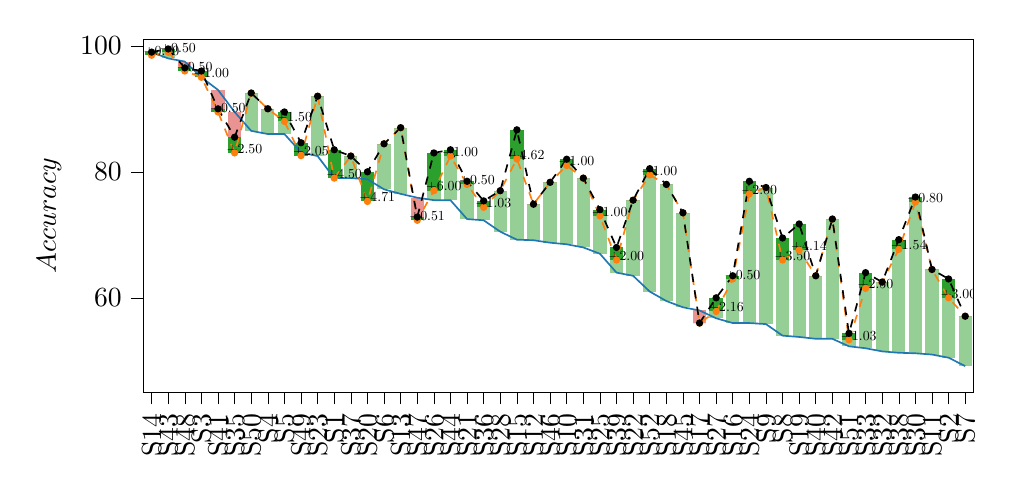
\begin{tikzpicture}

\definecolor{crimson2143940}{RGB}{214,39,40}
\definecolor{darkgray176}{RGB}{176,176,176}
\definecolor{darkorange25512714}{RGB}{255,127,14}
\definecolor{forestgreen4416044}{RGB}{44,160,44}
\definecolor{steelblue31119180}{RGB}{31,119,180}

\begin{axis}[
tick align=outside,
tick pos=left,
width=1\textwidth,
height=.5\textwidth,
x grid style={darkgray176},
xmin=-0.5, xmax=49.5,
xtick style={color=black},
xtick={0,1,2,3,4,5,6,7,8,9,10,11,12,13,14,15,16,17,18,19,20,21,22,23,24,25,26,27,28,29,30,31,32,33,34,35,36,37,38,39,40,41,42,43,44,45,46,47,48,49},
xticklabel style={rotate=90.0,anchor=east},
xticklabels={
  S14,
  S43,
  S48,
  S3,
  S41,
  S35,
  S50,
  S4,
  S5,
  S49,
  S23,
  S1,
  S37,
  S20,
  S6,
  S13,
  S47,
  S26,
  S44,
  S21,
  S36,
  S28,
  S15,
  S12,
  S46,
  S10,
  S31,
  S25,
  S39,
  S22,
  S52,
  S18,
  S45,
  S17,
  S27,
  S16,
  S24,
  S9,
  S8,
  S19,
  S40,
  S42,
  S51,
  S33,
  S32,
  S38,
  S30,
  S11,
  S2,
  S7,
},
y grid style={darkgray176},
ylabel={$Accuracy$},
ymin=45, ymax=101,
ytick style={color=black}
]
\draw[draw=none,fill=crimson2143940,fill opacity=0.5] (axis cs:-0.4,99) rectangle (axis cs:0.4,98.5);
\draw[draw=none,fill=forestgreen4416044,fill opacity=0.5] (axis cs:0.6,98) rectangle (axis cs:1.4,99);
\draw[draw=none,fill=crimson2143940,fill opacity=0.5] (axis cs:1.6,97.5) rectangle (axis cs:2.4,96);
\draw[draw=none,fill=crimson2143940,fill opacity=0.5] (axis cs:2.6,95) rectangle (axis cs:3.4,95);
\draw[draw=none,fill=crimson2143940,fill opacity=0.5] (axis cs:3.6,93) rectangle (axis cs:4.4,89.5);
\draw[draw=none,fill=crimson2143940,fill opacity=0.5] (axis cs:4.6,89.5) rectangle (axis cs:5.4,83);
\draw[draw=none,fill=forestgreen4416044,fill opacity=0.5] (axis cs:5.6,86.5) rectangle (axis cs:6.4,92.5);
\draw[draw=none,fill=forestgreen4416044,fill opacity=0.5] (axis cs:6.6,86) rectangle (axis cs:7.4,90);
\draw[draw=none,fill=forestgreen4416044,fill opacity=0.5] (axis cs:7.6,86) rectangle (axis cs:8.4,88);
\draw[draw=none,fill=crimson2143940,fill opacity=0.5] (axis cs:8.6,83.0769230769231) rectangle (axis cs:9.4,82.5641025641026);
\draw[draw=none,fill=forestgreen4416044,fill opacity=0.5] (axis cs:9.6,82.5) rectangle (axis cs:10.4,92);
\draw[draw=none,fill=crimson2143940,fill opacity=0.5] (axis cs:10.6,79) rectangle (axis cs:11.4,79);
\draw[draw=none,fill=forestgreen4416044,fill opacity=0.5] (axis cs:11.6,79) rectangle (axis cs:12.4,82.5);
\draw[draw=none,fill=crimson2143940,fill opacity=0.5] (axis cs:12.6,78.8235294117647) rectangle (axis cs:13.4,75.2941176470588);
\draw[draw=none,fill=forestgreen4416044,fill opacity=0.5] (axis cs:13.6,77.2222222222222) rectangle (axis cs:14.4,84.4444444444444);
\draw[draw=none,fill=forestgreen4416044,fill opacity=0.5] (axis cs:14.6,76.5) rectangle (axis cs:15.4,87);
\draw[draw=none,fill=crimson2143940,fill opacity=0.5] (axis cs:15.6,75.8974358974359) rectangle (axis cs:16.4,72.3076923076923);
\draw[draw=none,fill=forestgreen4416044,fill opacity=0.5] (axis cs:16.6,75.5) rectangle (axis cs:17.4,77);
\draw[draw=none,fill=forestgreen4416044,fill opacity=0.5] (axis cs:17.6,75.5) rectangle (axis cs:18.4,82.5);
\draw[draw=none,fill=forestgreen4416044,fill opacity=0.5] (axis cs:18.6,72.5) rectangle (axis cs:19.4,78);
\draw[draw=none,fill=forestgreen4416044,fill opacity=0.5] (axis cs:19.6,72.3076923076923) rectangle (axis cs:20.4,74.3589743589744);
\draw[draw=none,fill=forestgreen4416044,fill opacity=0.5] (axis cs:20.6,70.5) rectangle (axis cs:21.4,77);
\draw[draw=none,fill=forestgreen4416044,fill opacity=0.5] (axis cs:21.6,69.2307692307692) rectangle (axis cs:22.4,82.051282051282);
\draw[draw=none,fill=forestgreen4416044,fill opacity=0.5] (axis cs:22.6,69.1428571428572) rectangle (axis cs:23.4,74.8571428571429);
\draw[draw=none,fill=forestgreen4416044,fill opacity=0.5] (axis cs:23.6,68.75) rectangle (axis cs:24.4,78.3333333333333);
\draw[draw=none,fill=forestgreen4416044,fill opacity=0.5] (axis cs:24.6,68.5) rectangle (axis cs:25.4,81);
\draw[draw=none,fill=forestgreen4416044,fill opacity=0.5] (axis cs:25.6,68) rectangle (axis cs:26.4,79);
\draw[draw=none,fill=forestgreen4416044,fill opacity=0.5] (axis cs:26.6,67) rectangle (axis cs:27.4,73);
\draw[draw=none,fill=forestgreen4416044,fill opacity=0.5] (axis cs:27.6,64) rectangle (axis cs:28.4,66);
\draw[draw=none,fill=forestgreen4416044,fill opacity=0.5] (axis cs:28.6,63.5) rectangle (axis cs:29.4,75.5);
\draw[draw=none,fill=forestgreen4416044,fill opacity=0.5] (axis cs:29.6,61) rectangle (axis cs:30.4,79.5);
\draw[draw=none,fill=forestgreen4416044,fill opacity=0.5] (axis cs:30.6,59.5) rectangle (axis cs:31.4,78);
\draw[draw=none,fill=forestgreen4416044,fill opacity=0.5] (axis cs:31.6,58.5) rectangle (axis cs:32.4,73.5);
\draw[draw=none,fill=crimson2143940,fill opacity=0.5] (axis cs:32.6,58) rectangle (axis cs:33.4,56);
\draw[draw=none,fill=forestgreen4416044,fill opacity=0.5] (axis cs:33.6,56.7567567567568) rectangle (axis cs:34.4,57.8378378378379);
\draw[draw=none,fill=forestgreen4416044,fill opacity=0.5] (axis cs:34.6,56) rectangle (axis cs:35.4,63);
\draw[draw=none,fill=forestgreen4416044,fill opacity=0.5] (axis cs:35.6,56) rectangle (axis cs:36.4,76.5);
\draw[draw=none,fill=forestgreen4416044,fill opacity=0.5] (axis cs:36.6,55.8333333333333) rectangle (axis cs:37.4,77.5);
\draw[draw=none,fill=forestgreen4416044,fill opacity=0.5] (axis cs:37.6,54) rectangle (axis cs:38.4,66);
\draw[draw=none,fill=forestgreen4416044,fill opacity=0.5] (axis cs:38.6,53.7931034482759) rectangle (axis cs:39.4,67.5862068965517);
\draw[draw=none,fill=forestgreen4416044,fill opacity=0.5] (axis cs:39.6,53.5) rectangle (axis cs:40.4,63.5);
\draw[draw=none,fill=forestgreen4416044,fill opacity=0.5] (axis cs:40.6,53.5) rectangle (axis cs:41.4,72.5);
\draw[draw=none,fill=forestgreen4416044,fill opacity=0.5] (axis cs:41.6,52.3076923076923) rectangle (axis cs:42.4,53.3333333333333);
\draw[draw=none,fill=forestgreen4416044,fill opacity=0.5] (axis cs:42.6,52) rectangle (axis cs:43.4,61.5);
\draw[draw=none,fill=forestgreen4416044,fill opacity=0.5] (axis cs:43.6,51.5) rectangle (axis cs:44.4,62.5);
\draw[draw=none,fill=forestgreen4416044,fill opacity=0.5] (axis cs:44.6,51.2820512820513) rectangle (axis cs:45.4,67.6923076923077);
\draw[draw=none,fill=forestgreen4416044,fill opacity=0.5] (axis cs:45.6,51.2) rectangle (axis cs:46.4,75.2);
\draw[draw=none,fill=forestgreen4416044,fill opacity=0.5] (axis cs:46.6,51) rectangle (axis cs:47.4,64.5);
\draw[draw=none,fill=forestgreen4416044,fill opacity=0.5] (axis cs:47.6,50.5) rectangle (axis cs:48.4,60);
\draw[draw=none,fill=forestgreen4416044,fill opacity=0.5] (axis cs:48.6,49.1666666666667) rectangle (axis cs:49.4,57.0833333333333);
\draw[draw=none,fill=forestgreen4416044] (axis cs:-0.4,98.5) rectangle (axis cs:0.4,99);
\draw[draw=none,fill=forestgreen4416044] (axis cs:0.6,99) rectangle (axis cs:1.4,99.5);
\draw[draw=none,fill=forestgreen4416044] (axis cs:1.6,96) rectangle (axis cs:2.4,96.5);
\draw[draw=none,fill=forestgreen4416044] (axis cs:2.6,95) rectangle (axis cs:3.4,96);
\draw[draw=none,fill=forestgreen4416044] (axis cs:3.6,89.5) rectangle (axis cs:4.4,90);
\draw[draw=none,fill=forestgreen4416044] (axis cs:4.6,83) rectangle (axis cs:5.4,85.5);
\draw[draw=none,fill=crimson2143940] (axis cs:5.6,92.5) rectangle (axis cs:6.4,92.5);
\draw[draw=none,fill=crimson2143940] (axis cs:6.6,90) rectangle (axis cs:7.4,90);
\draw[draw=none,fill=forestgreen4416044] (axis cs:7.6,88) rectangle (axis cs:8.4,89.5);
\draw[draw=none,fill=forestgreen4416044] (axis cs:8.6,82.5641025641026) rectangle (axis cs:9.4,84.6153846153846);
\draw[draw=none,fill=crimson2143940] (axis cs:9.6,92) rectangle (axis cs:10.4,92);
\draw[draw=none,fill=forestgreen4416044] (axis cs:10.6,79) rectangle (axis cs:11.4,83.5);
\draw[draw=none,fill=crimson2143940] (axis cs:11.6,82.5) rectangle (axis cs:12.4,82.5);
\draw[draw=none,fill=forestgreen4416044] (axis cs:12.6,75.2941176470588) rectangle (axis cs:13.4,80);
\draw[draw=none,fill=crimson2143940] (axis cs:13.6,84.4444444444444) rectangle (axis cs:14.4,84.4444444444444);
\draw[draw=none,fill=crimson2143940] (axis cs:14.6,87) rectangle (axis cs:15.4,87);
\draw[draw=none,fill=forestgreen4416044] (axis cs:15.6,72.3076923076923) rectangle (axis cs:16.4,72.8205128205128);
\draw[draw=none,fill=forestgreen4416044] (axis cs:16.6,77) rectangle (axis cs:17.4,83);
\draw[draw=none,fill=forestgreen4416044] (axis cs:17.6,82.5) rectangle (axis cs:18.4,83.5);
\draw[draw=none,fill=forestgreen4416044] (axis cs:18.6,78) rectangle (axis cs:19.4,78.5);
\draw[draw=none,fill=forestgreen4416044] (axis cs:19.6,74.3589743589744) rectangle (axis cs:20.4,75.3846153846154);
\draw[draw=none,fill=crimson2143940] (axis cs:20.6,77) rectangle (axis cs:21.4,77);
\draw[draw=none,fill=forestgreen4416044] (axis cs:21.6,82.051282051282) rectangle (axis cs:22.4,86.6666666666667);
\draw[draw=none,fill=crimson2143940] (axis cs:22.6,74.8571428571429) rectangle (axis cs:23.4,74.8571428571429);
\draw[draw=none,fill=crimson2143940] (axis cs:23.6,78.3333333333333) rectangle (axis cs:24.4,78.3333333333333);
\draw[draw=none,fill=forestgreen4416044] (axis cs:24.6,81) rectangle (axis cs:25.4,82);
\draw[draw=none,fill=crimson2143940] (axis cs:25.6,79) rectangle (axis cs:26.4,79);
\draw[draw=none,fill=forestgreen4416044] (axis cs:26.6,73) rectangle (axis cs:27.4,74);
\draw[draw=none,fill=forestgreen4416044] (axis cs:27.6,66) rectangle (axis cs:28.4,68);
\draw[draw=none,fill=crimson2143940] (axis cs:28.6,75.5) rectangle (axis cs:29.4,75.5);
\draw[draw=none,fill=forestgreen4416044] (axis cs:29.6,79.5) rectangle (axis cs:30.4,80.5);
\draw[draw=none,fill=crimson2143940] (axis cs:30.6,78) rectangle (axis cs:31.4,78);
\draw[draw=none,fill=crimson2143940] (axis cs:31.6,73.5) rectangle (axis cs:32.4,73.5);
\draw[draw=none,fill=crimson2143940] (axis cs:32.6,56) rectangle (axis cs:33.4,56);
\draw[draw=none,fill=forestgreen4416044] (axis cs:33.6,57.8378378378378) rectangle (axis cs:34.4,60);
\draw[draw=none,fill=forestgreen4416044] (axis cs:34.6,63) rectangle (axis cs:35.4,63.5);
\draw[draw=none,fill=forestgreen4416044] (axis cs:35.6,76.5) rectangle (axis cs:36.4,78.5);
\draw[draw=none,fill=crimson2143940] (axis cs:36.6,77.5) rectangle (axis cs:37.4,77.5);
\draw[draw=none,fill=forestgreen4416044] (axis cs:37.6,66) rectangle (axis cs:38.4,69.5);
\draw[draw=none,fill=forestgreen4416044] (axis cs:38.6,67.5862068965517) rectangle (axis cs:39.4,71.7241379310345);
\draw[draw=none,fill=crimson2143940] (axis cs:39.6,63.5) rectangle (axis cs:40.4,63.5);
\draw[draw=none,fill=forestgreen4416044] (axis cs:40.6,72.5) rectangle (axis cs:41.4,72.5);
\draw[draw=none,fill=forestgreen4416044] (axis cs:41.6,53.3333333333333) rectangle (axis cs:42.4,54.3589743589744);
\draw[draw=none,fill=forestgreen4416044] (axis cs:42.6,61.5) rectangle (axis cs:43.4,64);
\draw[draw=none,fill=crimson2143940] (axis cs:43.6,62.5) rectangle (axis cs:44.4,62.5);
\draw[draw=none,fill=forestgreen4416044] (axis cs:44.6,67.6923076923077) rectangle (axis cs:45.4,69.2307692307692);
\draw[draw=none,fill=forestgreen4416044] (axis cs:45.6,75.2) rectangle (axis cs:46.4,76);
\draw[draw=none,fill=crimson2143940] (axis cs:46.6,64.5) rectangle (axis cs:47.4,64.5);
\draw[draw=none,fill=forestgreen4416044] (axis cs:47.6,60) rectangle (axis cs:48.4,63);
\draw[draw=none,fill=crimson2143940] (axis cs:48.6,57.0833333333333) rectangle (axis cs:49.4,57.0833333333333);
\addplot [semithick, steelblue31119180]
table {%
0 99
1 98
2 97.5
3 95
4 93
5 89.5
6 86.5
7 86
8 86
9 83.0769230769231
10 82.5
11 79
12 79
13 78.8235294117647
14 77.2222222222222
15 76.5
16 75.8974358974359
17 75.5
18 75.5
19 72.5
20 72.3076923076923
21 70.5
22 69.2307692307692
23 69.1428571428572
24 68.75
25 68.5
26 68
27 67
28 64
29 63.5
30 61
31 59.5
32 58.5
33 58
34 56.7567567567568
35 56
36 56
37 55.8333333333333
38 54
39 53.7931034482759
40 53.5
41 53.5
42 52.3076923076923
43 52
44 51.5
45 51.2820512820513
46 51.2
47 51
48 50.5
49 49.1666666666667
};
\addplot [semithick, darkorange25512714, mark=*, mark size=1, mark options={solid}, dashed]
table {%
0 98.5
1 99
2 96
3 95
4 89.5
5 83
6 92.5
7 90
8 88
9 82.5641025641026
10 92
11 79
12 82.5
13 75.2941176470588
14 84.4444444444444
15 87
16 72.3076923076923
17 77
18 82.5
19 78
20 74.3589743589744
21 77
22 82.051282051282
23 74.8571428571429
24 78.3333333333333
25 81
26 79
27 73
28 66
29 75.5
30 79.5
31 78
32 73.5
33 56
34 57.8378378378378
35 63
36 76.5
37 77.5
38 66
39 67.5862068965517
40 63.5
41 72.5
42 53.3333333333333
43 61.5
44 62.5
45 67.6923076923077
46 75.2
47 64.5
48 60
49 57.0833333333333
};
\addplot [semithick, black, mark=*, mark size=1, mark options={solid}, dashed]
table {%
0 99
1 99.5
2 96.5
3 96
4 90
5 85.5
6 92.5
7 90
8 89.5
9 84.6153846153846
10 92
11 83.5
12 82.5
13 80
14 84.4444444444444
15 87
16 72.8205128205128
17 83
18 83.5
19 78.5
20 75.3846153846154
21 77
22 86.6666666666667
23 74.8571428571429
24 78.3333333333333
25 82
26 79
27 74
28 68
29 75.5
30 80.5
31 78
32 73.5
33 56
34 60
35 63.5
36 78.5
37 77.5
38 69.5
39 71.7241379310345
40 63.5
41 72.5
42 54.3589743589744
43 64
44 62.5
45 69.2307692307692
46 76
47 64.5
48 63
49 57.0833333333333
};
\draw (axis cs:0.6,97.5) node[
  scale=0.5,
  anchor=south,
  text=black,
  rotate=0.0
]{+0.50};
\draw (axis cs:1.6,98) node[
  scale=0.5,
  anchor=south,
  text=black,
  rotate=0.0
]{+0.50};
\draw (axis cs:2.6,95) node[
  scale=0.5,
  anchor=south,
  text=black,
  rotate=0.0
]{+0.50};
\draw (axis cs:3.6,94) node[
  scale=0.5,
  anchor=south,
  text=black,
  rotate=0.0
]{+1.00};
\draw (axis cs:4.6,88.5) node[
  scale=0.5,
  anchor=south,
  text=black,
  rotate=0.0
]{+0.50};
\draw (axis cs:5.6,82) node[
  scale=0.5,
  anchor=south,
  text=black,
  rotate=0.0
]{+2.50};
\draw (axis cs:8.6,87) node[
  scale=0.5,
  anchor=south,
  text=black,
  rotate=0.0
]{+1.50};
\draw (axis cs:9.6,81.5641025641026) node[
  scale=0.5,
  anchor=south,
  text=black,
  rotate=0.0
]{+2.05};
\draw (axis cs:11.6,78) node[
  scale=0.5,
  anchor=south,
  text=black,
  rotate=0.0
]{+4.50};
\draw (axis cs:13.6,74.2941176470588) node[
  scale=0.5,
  anchor=south,
  text=black,
  rotate=0.0
]{+4.71};
\draw (axis cs:16.6,71.3076923076923) node[
  scale=0.5,
  anchor=south,
  text=black,
  rotate=0.0
]{+0.51};
\draw (axis cs:17.6,76) node[
  scale=0.5,
  anchor=south,
  text=black,
  rotate=0.0
]{+6.00};
\draw (axis cs:18.6,81.5) node[
  scale=0.5,
  anchor=south,
  text=black,
  rotate=0.0
]{+1.00};
\draw (axis cs:19.6,77) node[
  scale=0.5,
  anchor=south,
  text=black,
  rotate=0.0
]{+0.50};
\draw (axis cs:20.6,73.3589743589744) node[
  scale=0.5,
  anchor=south,
  text=black,
  rotate=0.0
]{+1.03};
\draw (axis cs:22.6,81.051282051282) node[
  scale=0.5,
  anchor=south,
  text=black,
  rotate=0.0
]{+4.62};
\draw (axis cs:25.6,80) node[
  scale=0.5,
  anchor=south,
  text=black,
  rotate=0.0
]{+1.00};
\draw (axis cs:27.6,72) node[
  scale=0.5,
  anchor=south,
  text=black,
  rotate=0.0
]{+1.00};
\draw (axis cs:28.6,65) node[
  scale=0.5,
  anchor=south,
  text=black,
  rotate=0.0
]{+2.00};
\draw (axis cs:30.6,78.5) node[
  scale=0.5,
  anchor=south,
  text=black,
  rotate=0.0
]{+1.00};
\draw (axis cs:34.6,56.8378378378378) node[
  scale=0.5,
  anchor=south,
  text=black,
  rotate=0.0
]{+2.16};
\draw (axis cs:35.6,62) node[
  scale=0.5,
  anchor=south,
  text=black,
  rotate=0.0
]{+0.50};
\draw (axis cs:36.6,75.5) node[
  scale=0.5,
  anchor=south,
  text=black,
  rotate=0.0
]{+2.00};
\draw (axis cs:38.6,65) node[
  scale=0.5,
  anchor=south,
  text=black,
  rotate=0.0
]{+3.50};
\draw (axis cs:39.6,66.5862068965517) node[
  scale=0.5,
  anchor=south,
  text=black,
  rotate=0.0
]{+4.14};
\draw (axis cs:42.6,52.3333333333333) node[
  scale=0.5,
  anchor=south,
  text=black,
  rotate=0.0
]{+1.03};
\draw (axis cs:43.6,60.5) node[
  scale=0.5,
  anchor=south,
  text=black,
  rotate=0.0
]{+2.50};
\draw (axis cs:45.6,66.6923076923077) node[
  scale=0.5,
  anchor=south,
  text=black,
  rotate=0.0
]{+1.54};
\draw (axis cs:46.6,74.2) node[
  scale=0.5,
  anchor=south,
  text=black,
  rotate=0.0
]{+0.80};
\draw (axis cs:48.6,59) node[
  scale=0.5,
  anchor=south,
  text=black,
  rotate=0.0
]{+3.00};
\end{axis}

\end{tikzpicture}}
%   \caption{Comparison of subject-specific average accuracy across EEGnet, KCS-FCnet, and RKCS-FCnet models. Subjects are arranged in descending order based on the accuracy of the EEGnet model. The color-coded bars illustrate performance shifts, with dark green(\legend{forestgreen4416044}) indicating an increase in accuracy on the RKCS-FCnet over KCS-FCnet, light green(\legend{forestgreen4416044!50}) indicating an increase in accuracy on KCS-FCnet over EEGnet, and while red \legend{crimson2143940!50} indicates an accuracy reduction.}\label{fig:accuracy_sbj_comp}
% \end{figure}


% It seems some of the future work in the conclusion directly contradicts what was said earlier about avoiding complexity of graph neural networks. Perhaps those earlier comments could be tempered.
% R// thank you for the valuable comment, we agree and change the paragraph:
%  \changes{While Graph Neural Networks are capable of managing complex graph-structured data, they can be computationally demanding due to the necessity of processing all nodes and their neighbors within the graph. However, ongoing advancements in optimization techniques are continually improving their efficiency \cite{gao2024graph}.}



% Minor style issue throuhgout: 

% Units like mV, V, and Hz are not italics. Nor should reference names be italics. "Table X", "Figure X", "Section X", etc. should be capitalized and not abbreviated like in Chapter 6, but consistent throughout.  

% R// thank you for the recommendation we removed all italics refering to Units and names. Also "Table X", "Figure X", "Section X" was changed as suggested.


 
\end{reviewer}

\clearpage
\bibliographystyle{splncs04}
\bibliography{../Tesis_document/References}

\end{document}


